% A LaTeX template for ARTICLE version of the MSc Thesis submissions to 
% Politecnico di Milano (PoliMi) - School of Industrial and Information Engineering
%
% S. Bonetti, A. Gruttadauria, G. Mescolini, A. Zingaro
% e-mail: template-tesi-ingind@polimi.it
%
% Last Revision: October 2021
%
% Copyright 2021 Politecnico di Milano, Italy. Inc. NC-BY

\documentclass[11pt,a4paper]{article} 

%------------------------------------------------------------------------------
%	REQUIRED PACKAGES AND  CONFIGURATIONS
%------------------------------------------------------------------------------
% PACKAGES FOR TITLES
\usepackage{titlesec}
\usepackage{color}

% PACKAGES FOR LANGUAGE AND FONT
\usepackage[utf8]{inputenc}
\usepackage[english]{babel}
\usepackage[T1]{fontenc} % Font encoding

% PACKAGES FOR IMAGES
\usepackage{graphicx}
\graphicspath{{Images/}}
\usepackage{eso-pic} % For the background picture on the title page
\usepackage{subfig} % Numbered and caption subfigures using \subfloat
\usepackage{caption} % Coloured captions
\usepackage{transparent}

% STANDARD MATH PACKAGES
\usepackage{amsmath}
\usepackage{amssymb}
\usepackage{amsthm}
\usepackage{bm}
\usepackage[overload]{empheq}  % For braced-style systems of equations

% PACKAGES FOR TABLES
\usepackage{tabularx}
\usepackage{longtable} % tables that can span several pages
\usepackage{booktabs} % Professional table rules like \toprule
\usepackage{colortbl}

% PACKAGES FOR ALGORITHMS (PSEUDO-CODE)
\usepackage{algorithm}
\usepackage{algorithmic}

% PACKAGES FOR REFERENCES & BIBLIOGRAPHY
\usepackage[colorlinks=true,linkcolor=black,anchorcolor=black,citecolor=black,filecolor=black,menucolor=black,runcolor=black,urlcolor=black]{hyperref} % Adds clickable links at references
\usepackage{cleveref}
\usepackage[square, numbers, sort&compress]{natbib} % Square brackets, citing references with numbers, citations sorted by appearance in the text and compressed
\bibliographystyle{plain} % You may use a different style adapted to your field

% PACKAGES FOR THE APPENDIX
\usepackage{appendix}

% PACKAGES FOR ITEMIZE & ENUMERATES 
\usepackage{enumitem}

% OTHER PACKAGES
\usepackage{amsthm,thmtools,xcolor} % Coloured "Theorem"
\usepackage{comment} % Comment part of code
\usepackage{fancyhdr} % Fancy headers and footers
\usepackage{lipsum} % Insert dummy text
\usepackage{tcolorbox} % Create coloured boxes (e.g. the one for the key-words)

%-------------------------------------------------------------------------
%	NEW COMMANDS DEFINED
%-------------------------------------------------------------------------
% EXAMPLES OF NEW COMMANDS -> here you see how to define new commands
\newcommand{\bea}{\begin{eqnarray}} % Shortcut for equation arrays
\newcommand{\eea}{\end{eqnarray}}
\newcommand{\e}[1]{\times 10^{#1}}  % Powers of 10 notation
\newcommand{\mathbbm}[1]{\text{\usefont{U}{bbm}{m}{n}#1}} % From mathbbm.sty
\newcommand{\pdev}[2]{\frac{\partial#1}{\partial#2}}
% NB: you can also override some existing commands with the keyword \renewcommand

%----------------------------------------------------------------------------
%	ADD YOUR PACKAGES (be careful of package interaction)
%----------------------------------------------------------------------------
\usepackage{etoolbox}
\AtBeginEnvironment{equation}{\small}
\AtBeginEnvironment{align}{\small}
\AtBeginEnvironment{equation*}{\small}
\AtBeginEnvironment{align*}{\small}

%----------------------------------------------------------------------------
%	ADD YOUR DEFINITIONS AND COMMANDS (be careful of existing commands)
%----------------------------------------------------------------------------


% Do not change Configuration_files/config.tex file unless you really know what you are doing. 
% This file ends the configuration procedures (e.g. customizing commands, definition of new commands)
\input{Configuration_files/config}

% Insert here the info that will be displayed into your Title page 
% -> title of your work
\renewcommand{\title}{054702 - AUTOMATION AND CONTROL LABORATORY}
% -> author name and surname
\newcommand{\authora}{Negm Karim}
\newcommand{\authorb}{Hu Kaipeng}
\newcommand{\authorc}{Yan Yawen}
\newcommand{\authord}{Zeep Nathan}
% -> MSc course
\newcommand{\course}{Seesaw}
% -> advisor name and surname
\newcommand{\advisor}{Prof. Ruiz Fredy}
% IF AND ONLY IF you need to modify the co-supervisors you also have to modify the file Configuration_files/title_page.tex (ONLY where it is marked)
\newcommand{\firstcoadvisor}{Cordoba Andres} % insert if any otherwise comment
% -> author ID
\newcommand{\IDa}{11063520}
\newcommand{\IDb}{11036887}
\newcommand{\IDc}{11015522}
\newcommand{\IDd}{10977678}
% -> academic year
\newcommand{\YEAR}{2025-2026}
% -> abstract (only in English)
\renewcommand{\abstract}{This thesis presents the design and implementation of a state-space control system for a Quanser Seesaw platform. The work includes system identification, the design of a pole-placement controller with integral action, and the implementation of a Luenberger observer for state estimation. Performance is validated through linear simulation and hardware experiments, demonstrating robust stabilization and disturbance rejection.}

% -> key-words (only in English)
\newcommand{\keywords}{Control, Model, Seesaw}

%-------------------------------------------------------------------------
%	BEGIN OF YOUR DOCUMENT
%-------------------------------------------------------------------------
\begin{document}

%-----------------------------------------------------------------------------
% TITLE PAGE
%-----------------------------------------------------------------------------
% Do not change Configuration_files/TitlePage.tex (Modify it IF AND ONLY IF you need to add or delete the Co-advisors)
% This file creates the Title Page of the document
% DO NOT REMOVE SPACES BETWEEN LINES!

\AddToShipoutPicture*{\BackgroundPic}

\hspace{-0.6cm}
\includegraphics[width=0.6\textwidth]{logo_polimi_ing_indinf.eps}

\vspace{-1mm}
\Large{\textbf{\color{bluePoli}{\title}}}\\

\vspace{-0.2cm}

\begin{center}
\begin{minipage}[t]{.44\textwidth}
\fontsize{0.6cm}{0.5cm}\selectfont \bfseries \textsc{\color{bluePoli} Laboratory Report for the setup: \course}\\

\vspace{-0.2cm}
\large{\textbf{\authora, \IDa}}\\
\large{\textbf{\authorb, \IDb}}\\
\large{\textbf{\authorc, \IDc}}\\
\large{\textbf{\authord, \IDd}}
\end{minipage}
\begin{minipage}[t]{.54\textwidth}
\raggedleft
\Large{\textbf{Supervisors:}} \\
\large{\advisor} \\
%\\
%\textbf{Co-advisors:} \\ % leave it if any co-advisor otherwise comment
\large{\firstcoadvisor} \\ % leave it if you have more that one co-advisor otherwise comment (if you have more than two co-advisors just copy&paste this line writing \thirdcoadvisor, \fourthcoadvisor, ecc. (REMEMBER to modify also the main.txt)
\vspace{0.2cm} % leave it if any co-advisor otherwise comment
\Large{\textbf{Academic year:}} \\
\large{\YEAR} \\
\vspace{0.2cm}
\end{minipage}
\end{center}

\vspace{15pt}

\begin{tcolorbox}[arc=0pt, boxrule=0pt, colback=bluePoli!60, width=\textwidth, colupper=white]
    \textbf{Key-words:} \keywords
\end{tcolorbox}

\vspace{12pt}

%%%%%%%%%%%%%%%%%%%%%%%%%%%%%%
%%     THESIS MAIN TEXT     %%
%%%%%%%%%%%%%%%%%%%%%%%%%%%%%%

\section{Introduction}

\section{Setups Descriptions}

\subsection{Cart Subsystem}
The cart is a 1-DOF linear system. Parameters are derived from the hardware datasheet and validated experimentally in Section~\ref{sec:tuning}.

The actual weight of the cart seen by the motor is
\begin{equation}
	M_e = M_c + \frac{J_m \cdot K_g^2}{r_{mp}^2}
\end{equation}
Defining the force acting on the cart as
\begin{equation}
	F_c(t) = \alpha \cdot v(t) - B_{emf} \cdot \dot{x}_c(t)
\end{equation}
where
\begin{align*}
	\alpha  & = \frac{k_tK_g\eta_g\eta_m}{r^2_{mp}R_m} &
	B_{emf} & = \frac{k_tk_mK^2_g\eta_g}{r^2_{mp}R_m}
\end{align*}

The kinetic energy takes the form
\begin{equation}
	T = \frac{1}{2}M_e\dot{x}_c^2
\end{equation}
The equation of motion of the system is:
\begin{equation}
	\label{eq:cart_eom}
	\begin{aligned}
		                & \frac{\partial^2T}{\partial t \partial \dot{x}_c} - \frac{\partial T}{\partial x_c} & = & -B_{eq,c} \cdot \dot{x}_c + F_c                                     \\
		\Leftrightarrow & M_e \cdot \ddot{x}_c                                                                & = & -B_{eq,c} \cdot \dot{x}_c + \alpha \cdot v - B_{emf}\cdot \dot{x}_c \\
		\Leftrightarrow & M_e \cdot \ddot{x}_c(t) + (B_{eq,c} + B_{emf}) \cdot \dot{x}_c (t)                  & = & \alpha \cdot v(t)
	\end{aligned}
\end{equation}

\subsection{Seesaw and Cart System}
The coupled 2-DOF system consists of cart position $x_c$ and seesaw inclination $\theta$. The Lagrangian $L = T - V$ is used to derive the equations of motion.
\begin{equation}
	T = \frac{1}{2}M_e \dot{x}_c^2 + \frac{1}{2}(J_{sw} + M_eD_T^2)\dot{\theta}^2 + \frac{1}{2}M_ex_c^2 \dot{\theta}^2 - M_eD_T \dot{x}_c \dot{\theta}
\end{equation}
\begin{equation}
	V = gM_ex_csin(\theta) + g(M_eD_T + M_{sw}D_C )cos(\theta)
\end{equation}
Using the Euler-Lagrange relation:\\
\begin{equation}
	\left\{
	\begin{aligned}
		\frac{\partial^2L}{\partial t \partial \dot{x}_c} - \frac{\partial L}{\partial x_c}       & = - B_{eq,c} \dot{x}_c + F_c \\
		\frac{\partial^2L}{\partial t \partial \dot{\theta}} - \frac{\partial L}{\partial \theta} & = - B_{sw} \dot{\theta}
	\end{aligned}
	\right.
\end{equation}
The final equations of motion for the complete system are:
\begin{equation}
	\label{eq:seesaw_eom}
	\left\{
	\begin{aligned}
		M_e\dot{x}_c - M_eD_T \ddot{\theta} - M_e x_c \dot{\theta}^2 + gM_e sin(\theta)                 & = - B_{eq,c} \dot{x}_c + F_c \\
		M_e \ddot{\theta} x_c^2 + 2M_e \dot{x}_c \dot{\theta} + gM_ecos(\theta)x_c - M_e D_T \ddot{x}_c & +                            \\
		(J_{sw} + M_eD^2_T)\ddot{\theta} - g(M_eD_T - M_{sw}D_C)sin(\theta)                             & = - B_{sw} \dot{\theta}
	\end{aligned}
	\right.
\end{equation}

\section{First experience: Cart position control}

\subsection{Transfer Function Definition}

Based on the equation of motion described at Eq.~\ref{eq:cart_eom}, we define the transfer function of the system using the Laplace Transform.
\begin{equation}
	\label{eq:cart_eom_laplace}
	[M_e \cdot s^2 + (B_{eq,c} + B_{emf}) \cdot s]\cdot X_c(s) = \alpha \cdot V(s)
\end{equation}
\begin{equation}
	\label{eq:cart_tf}
	\begin{aligned}
		G(s) = \frac{X(s)}{V(s)} & = \frac{\alpha}{M_e \cdot s^2 + B_{tot} \cdot s}                           \\
		                         & = \frac{1}{s} \cdot \frac{(\alpha / B_{tot})}{(M_e / B_{tot}) \cdot s + 1}
	\end{aligned}
\end{equation}

\subsection{System Identification and Tuning} \label{sec:tuning}
Parameters $B_{eq,c}$, $\eta_g$, and $\eta_m$ are identified through experimental data fitting. Nominal values from Table~\ref{table:datasheet} serve as initial estimates.
\begin{comment}

	\paragraph{Motor inductance ($L_m$)}
Assuming $L_m \approx 0$ simplifies the plant from 3rd to 2nd order. This is justified as the electrical pole is at $\sim 1.4 \times 10^4$ rad/s, three orders of magnitude above the mechanical bandwidth.
\end{comment}
\paragraph{Friction and Efficiency Tuning}
Viscous coefficient $B_{eq,c}$ is identified via sine-sweep excitation and mean-square error fitting. Efficiencies $\eta_g$ and $\eta_m$ are tuned using step-response time constants and DC gain. A grid search identifies values that account for unmodelled Coulomb friction and cable drag.

$\tau = \frac{M_e}{B_{tot}(\eta_g)}, \qquad K = \frac{\alpha (\eta_g,\eta_m)}{B_{tot}(\eta_g)}$

\begin{table}[H]
	%\caption*{\textbf{Example of Table (optional)}}
	\centering
	% Use tabularx with \textwidth. The 'X' column will stretch.
	\begin{tabularx}{\textwidth}{|X c c c |}
		\hline
		\rowcolor{bluePoli!40}
		                              & \textbf{$\eta_g$} & \textbf{$\eta_m$} & \textbf{mean square error} \T\B \\
		\hline \hline
		\textbf{datasheet base value} & $0.9$             & $0.69$            & $1.11\cdot 10^2$ \T\B           \\
		\textbf{datasheet variation}  & $0.81$            & $0.65$            & $8.08\cdot 10^1$ \T\B           \\
		\textbf{extra variation}      & $0.72$            & $0.5865$          & $4.98\cdot 10^1$ \B             \\
		\hline
	\end{tabularx}
	\\[10pt]
	\caption{Efficiencies and associated MSE depending on the setup.}
	\label{table:datasheet}
\end{table}

The identified model parameters that provide the best fit to the measured step response are $B_{eq,c}=3.87$, $\eta_g = 0.6$, and $\eta_m =0.69$ (see Fig.~\ref{fig:comp}).

\begin{figure}
	\centering
	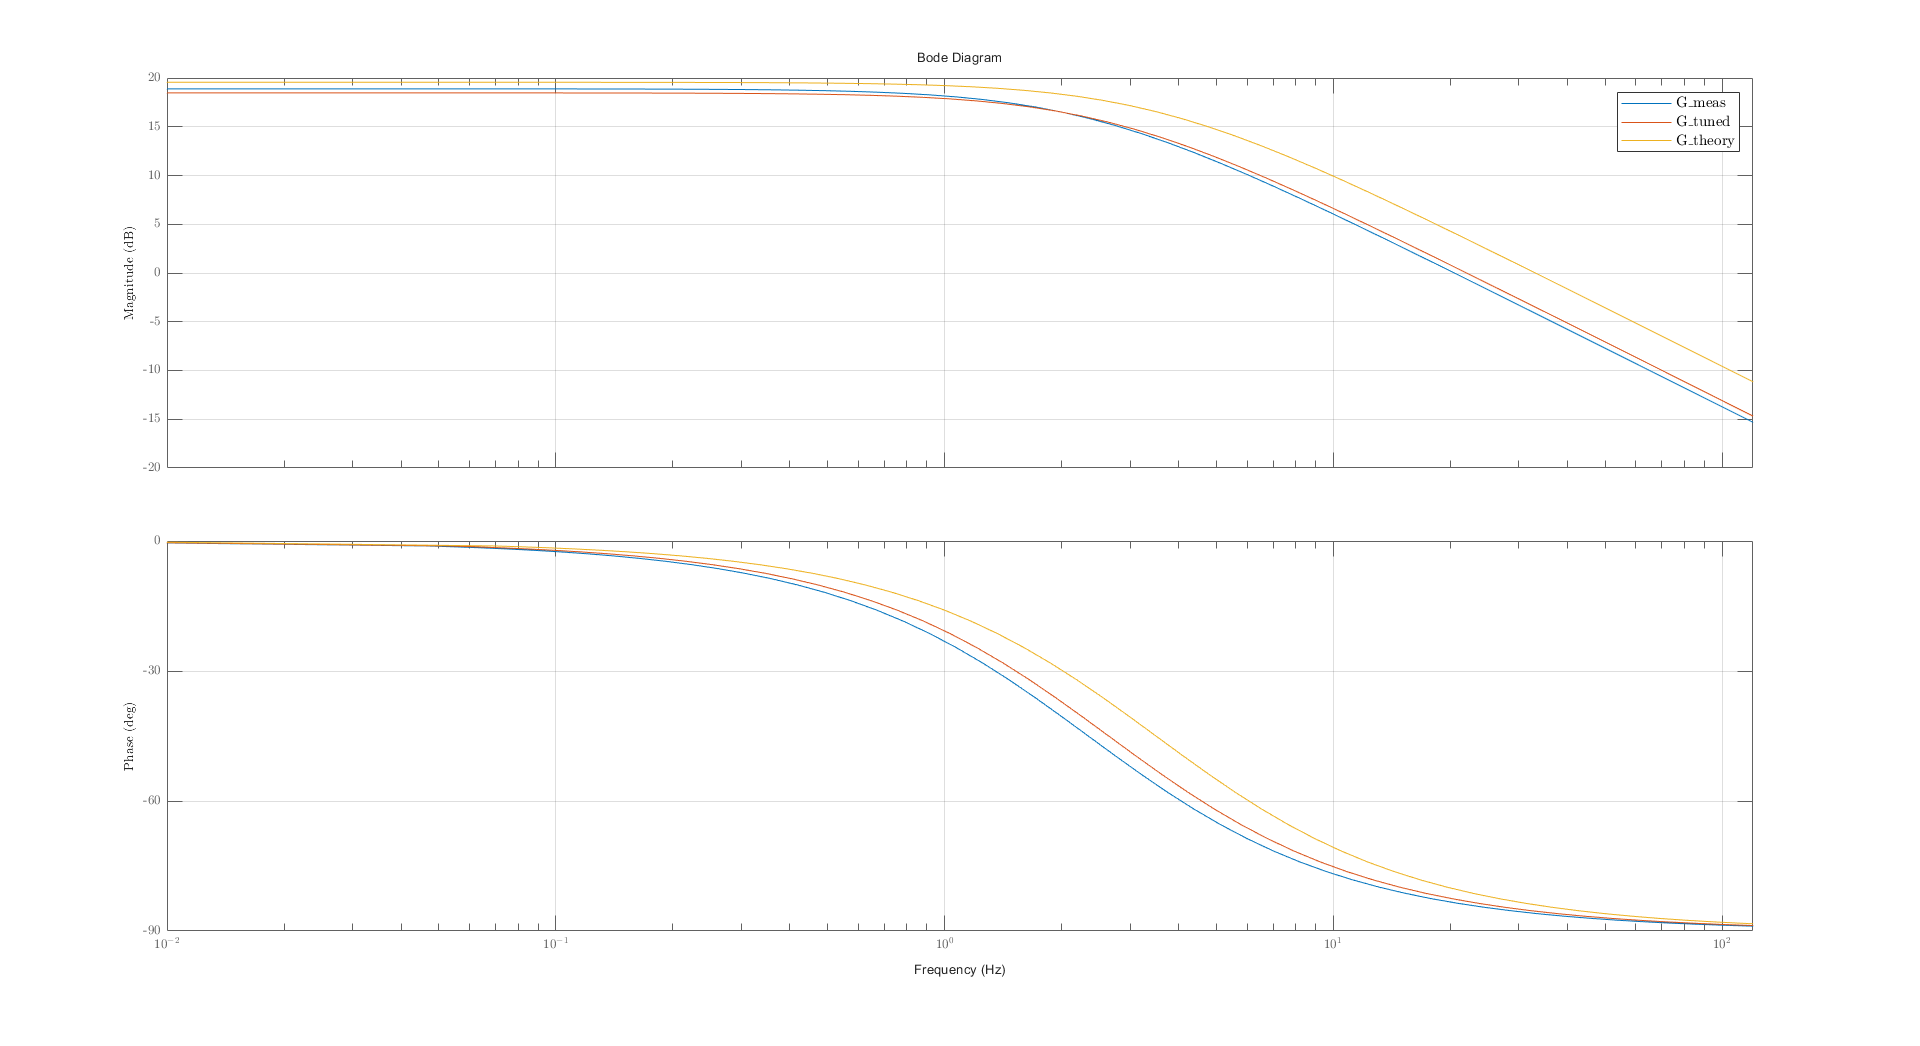
\includegraphics[width=0.7\linewidth]{Images/bode_comparison_meas_tuned_theory.png}
	\caption{Caption}
	\label{fig:comp}
\end{figure}

\begin{figure}[H]
	\centering
	\subfloat[One PoliMi logo.\label{fig:polimi_logo1}]{
		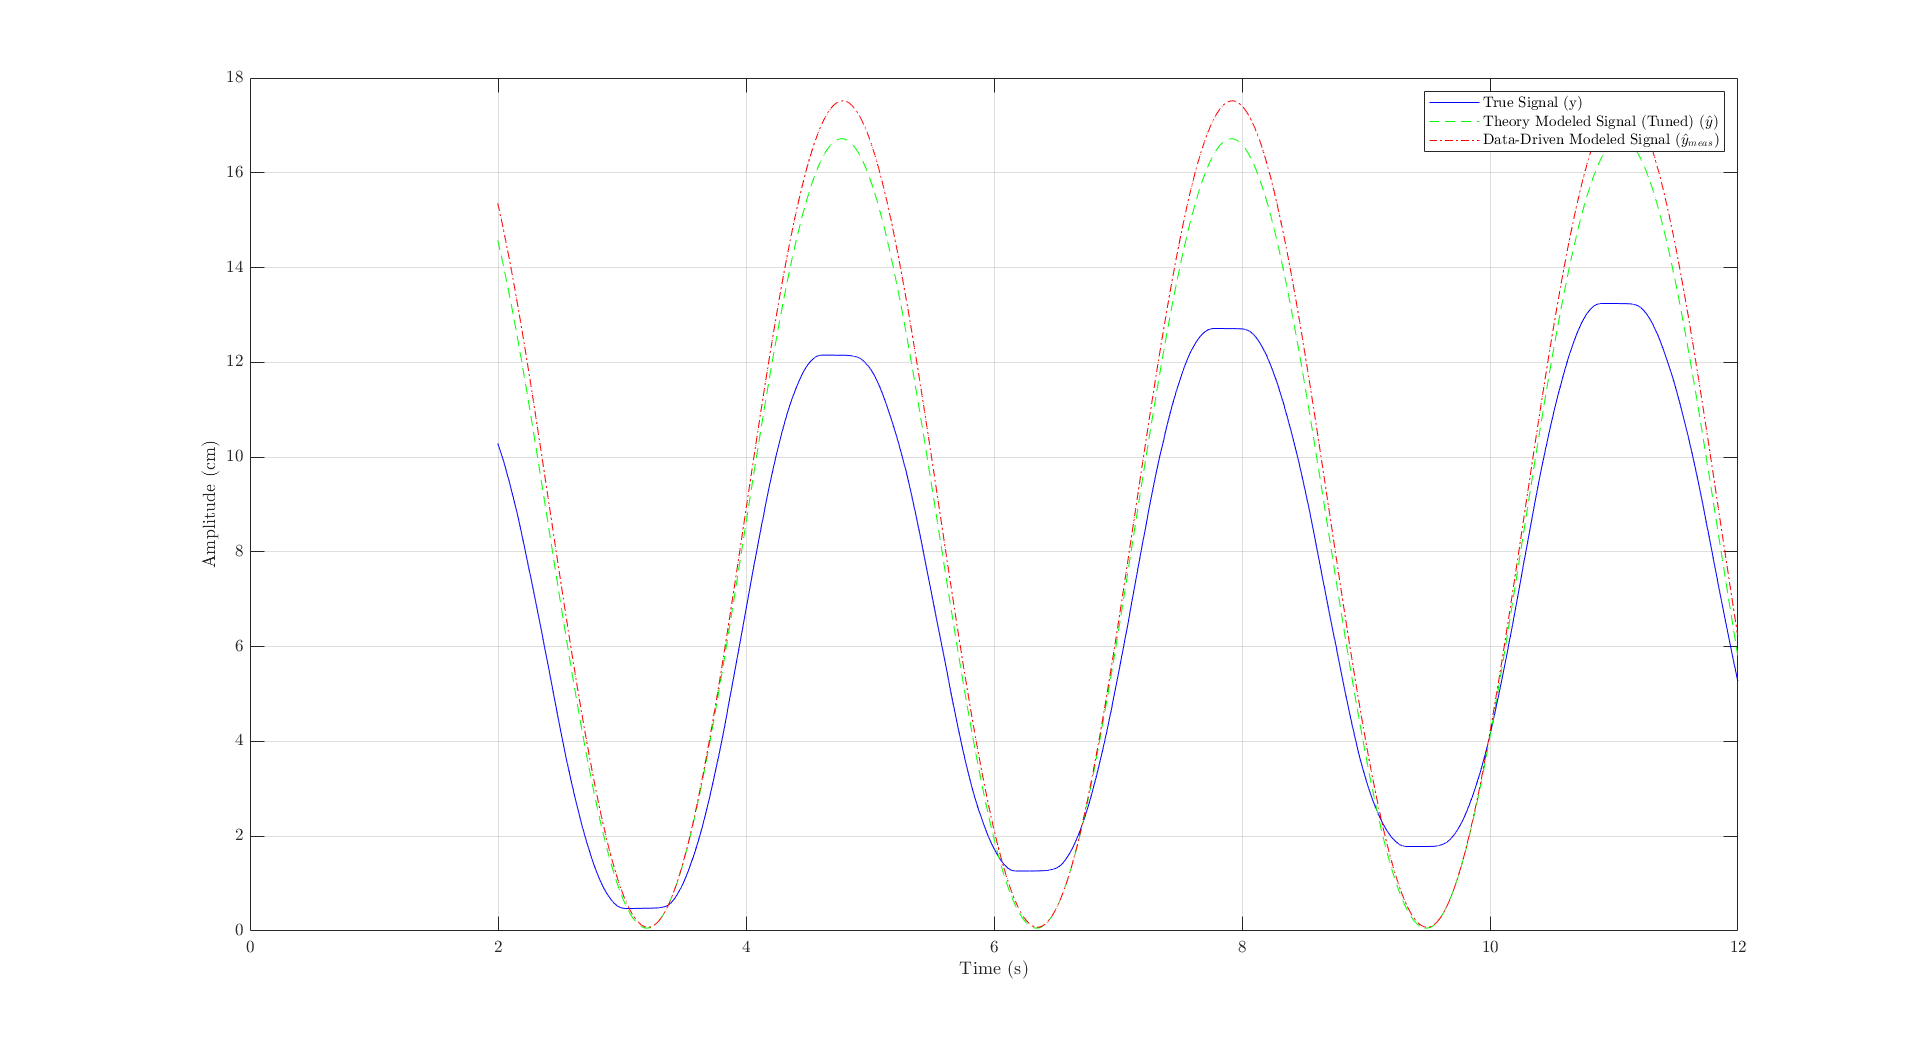
\includegraphics[width=0.4\linewidth]{Images/time_comparison_2hz_real_tuned_meas.png}
	}
	\quad
	\subfloat[Another one PoliMi logo.\label{fig:polimi_logo2}]{
		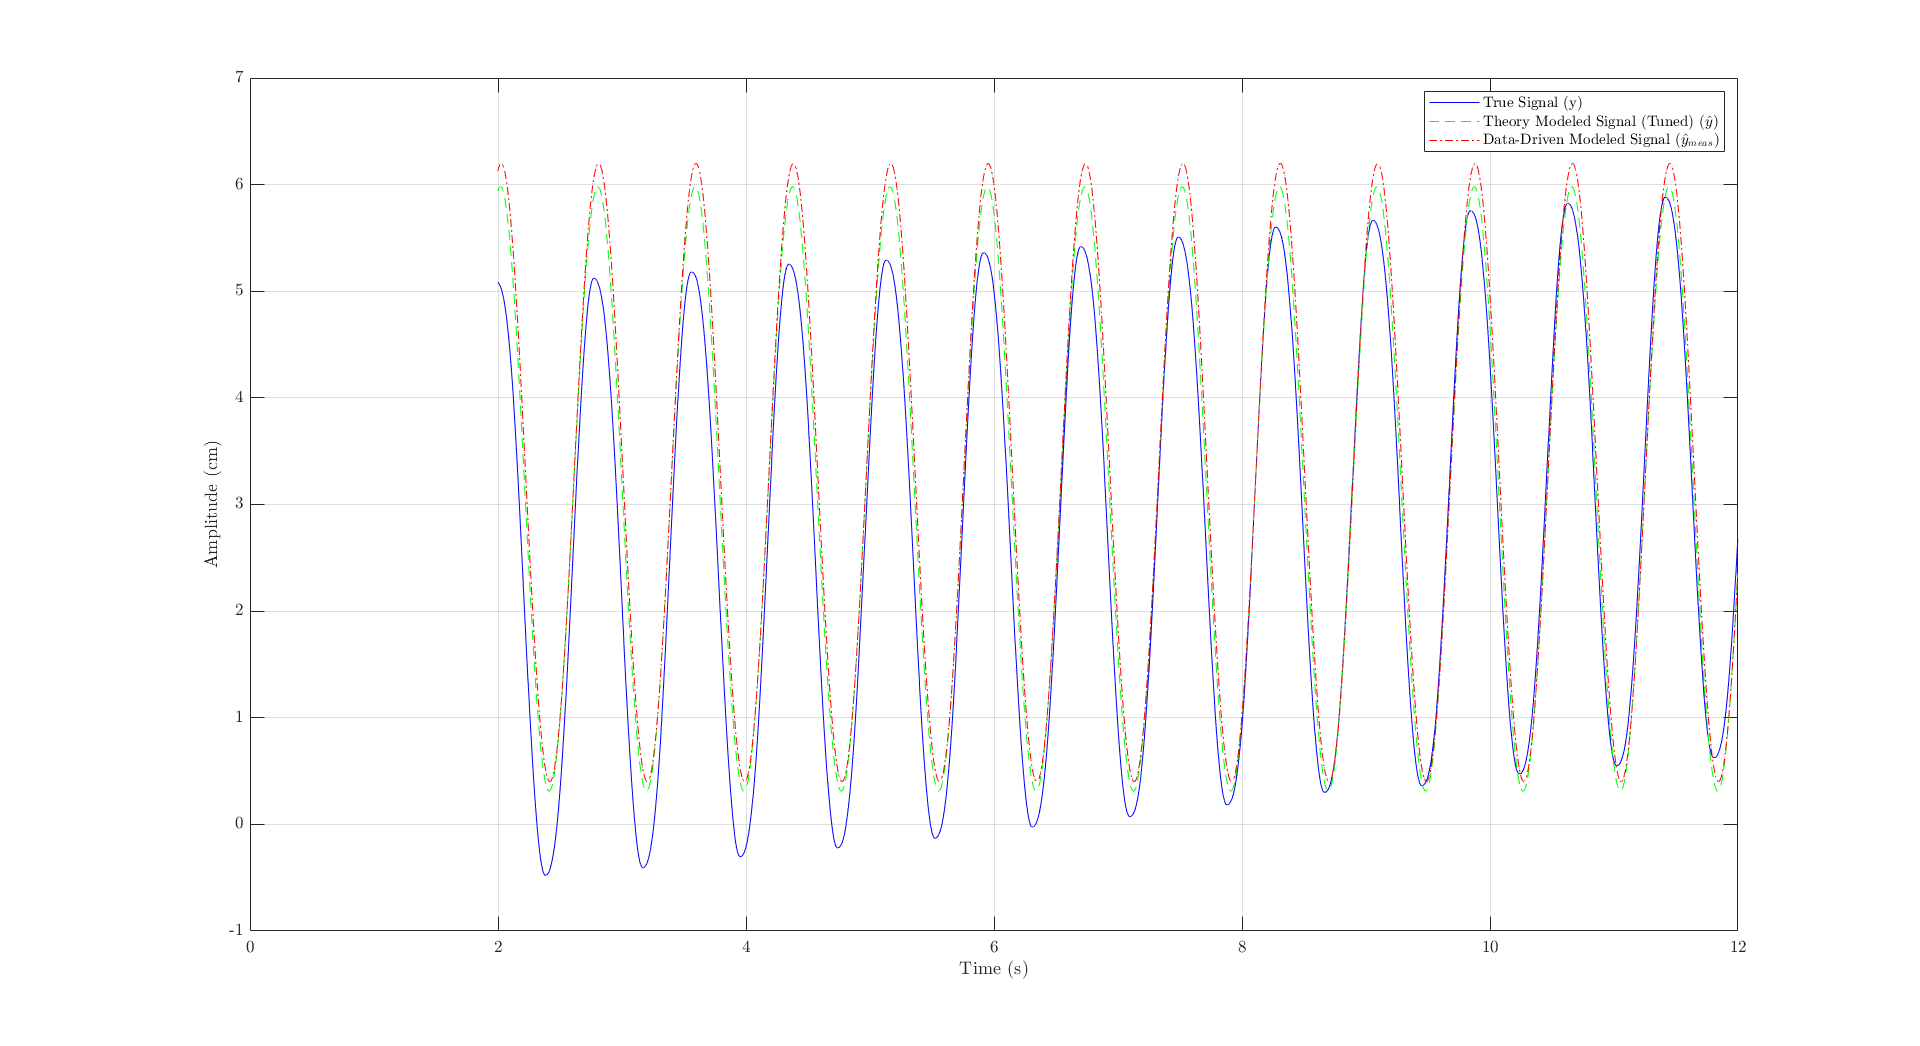
\includegraphics[width=0.4\linewidth]{Images/time_comparison_8hz_real_tuned_meas.png}
	}
	\caption[]{Caption of the Figure.}
	\label{fig:quadtree2}
\end{figure}

final values $\eta_g = 0.72$ [-], $\eta_m = 0.5865$ [-]\\

\subsection{Model Validation}

\paragraph{Time validation}

\paragraph{Frequency Validation}

\subsection{Control of the position}

using PID control

\section{Second experience: Body Stabilization in horizontal position}

\subsection{Transfer Functions Definition}

Assumptions for linearization :
\begin{enumerate}
	\item Small angles ($\theta \simeq 0$) : $sin(\theta) = \theta$ and $cos(\theta) = 1$
	\item Ignoring high-order velocity terms : $\dot{\theta}^2, x_c^2, \dot{x}_c\dot{\theta} \simeq 0$
\end{enumerate}
After linearizing and replacing $F_c$, the system is:
\begin{equation}
	\left\{
	\begin{aligned}
		M_e\dot{x}_c - M_eD_T \ddot{\theta}
		+ gM_e \theta + B_c \dot{x}_c + B_{emf}\dot{x}_c & =  \alpha V_{DC} \\
		- M_e D_T \ddot{x}_c + gM_ex_c +                                    \\ (J_{sw} + M_eD^2_T)\ddot{\theta} + B_{sw} \dot{\theta} - g(M_eD_T - M_{sw}D_C)\theta &= 0
	\end{aligned}
	\right.
\end{equation}
For which the Laplace trasnform gives, considering initial states of (0,0):
\begin{equation}
	\left\{
	\begin{aligned}
		(M_e s^2 + (B_{eq,c} + B_{emf})s) \cdot X(s)                                & +                         \\
		(- M_e D_T s^2 + g M_e s) \cdot \Theta (s)                                  & =  \alpha \cdot V_{DC}(s) \\
		(-M_e D_T s^2 + g M_e) \cdot X(s)                                           & +                         \\
		( (J_{sw} + M_e D_T)s^2 + B_{sw}s - g(M_eD_T + M_{sw}D_C)) \cdot \Theta (s) & = 0
	\end{aligned}
	\right.
\end{equation}

Matrix form :
\begin{equation}
	\begin{bmatrix}
		M_e s^2 + (B_{eq,c} + B_{emf})s & -M_e D_T s^2 + g M_e s                                  \\
		-M_e D_T s^2 + g M_e            & (J_{sw} + M_e D_T)s^2 + B_{sw}s - g(M_eD_T + M_{sw}D_C)
	\end{bmatrix}
	\begin{bmatrix}
		X(s) \\
		\Theta(s)
	\end{bmatrix}
	=
	\begin{bmatrix}
		\alpha \\
		0
	\end{bmatrix}
	V_{DC}(s)
\end{equation}
\begin{equation}
	\begin{bmatrix}
		P_{11} & P_{12} \\
		P_{21} & P_{22}
	\end{bmatrix}
	\begin{bmatrix}
		X(s) \\
		\Theta(s)
	\end{bmatrix}
	=
	\begin{bmatrix}
		\alpha \\
		0
	\end{bmatrix}
	V_{DC}(s)
\end{equation}
using Cramer's rule we can define $G(s)$ and $H(s)$ the transfer functions from $V_{DC}(s)$ to respectively $X(s)$ and $\Theta(s)$.
\begin{equation}
	\begin{aligned}
		G(s) & = \frac{X(s)}{V_{DC}(s)}      & = \alpha \frac{P_{22}}{P_{11}\cdot P_{22} - P_{12} \cdot P_{21}}  \\
		     &                               & = \frac{numG}{den}                                                \\
		H(s) & = \frac{\Theta(s)}{V_{DC}(s)} & = \alpha \frac{-P_{21}}{P_{11}\cdot P_{22} - P_{12} \cdot P_{21}} \\
		     &                               & = \frac{numH}{den}
	\end{aligned}
\end{equation}

Both share the same 4 poles : \textcolor{red}{$-23, \quad -3.31, \quad 0, \quad 3$}\\
Having the 4\textsuperscript{th} pole positive makes the system unstable and this requires the control actions developed in the next sections.

\subsection{State-Space Representation}
Solving the equations of motions for the second order derivative:
\begin{equation}
	\begin{bmatrix}
		M_e     & -M_eD_T           \\
		-M_eD_T & J_{sw} + M_eD_T^2
	\end{bmatrix}
	\begin{bmatrix}
		\ddot{x}_c \\
		\ddot{\theta}
	\end{bmatrix}
	=
	\begin{bmatrix}
		0     & -gM_e                 & -B_{tot} & 0       \\
		-gM_e & g(M_eD_T + M_{sw}D_C) & 0        & -B_{sw}
	\end{bmatrix}
	\begin{bmatrix}
		x_c       \\
		\theta    \\
		\dot{x}_c \\
		\dot{\theta}
	\end{bmatrix}
	+ \begin{bmatrix}
		\alpha \\
		0
	\end{bmatrix}
	V
\end{equation}
\begin{comment}
	\begin{equation}
		\begin{aligned}
			\begin{bmatrix}
				\ddot{x}_c \\
				\ddot{\theta}
			\end{bmatrix}
			 & =
			\frac{1}{M_eJ_{sw}}
			\begin{bmatrix}
				J_{sw} + M_eD_T^2 & M_eD_T \\
				M_eD_T            & M_e
			\end{bmatrix}
			\begin{bmatrix}
				0     & -gM_e                 & -B_{tot} & 0       \\
				-gM_e & g(M_eD_T + M_{sw}D_C) & 0        & -B_{sw}
			\end{bmatrix}
			\begin{bmatrix}
				x_c       \\
				\theta    \\
				\dot{x}_c \\
				\dot{\theta}
			\end{bmatrix} \\
			 & +
			\frac{1}{M_eJ_{sw}}
			\begin{bmatrix}
				J_{sw} + M_eD_T^2 & M_eD_T \\
				M_eD_T            & M_e
			\end{bmatrix}
			\begin{bmatrix}
				\alpha \\
				0
			\end{bmatrix}
			V
		\end{aligned}
	\end{equation}

\end{comment}
\begin{equation}
	\begin{aligned}
		\begin{bmatrix}
			\ddot{x}_c \\
			\ddot{\theta}
		\end{bmatrix}
		 & =
		\frac{1}{J_{sw}}
		\begin{bmatrix}
			-gM_eD_T & g( -J_{sw} + 2gM_eD_T^2 + M_{sw}D_TD_C) & -B_{tot}(\frac{J_{sw}}{M_e}+D_T^2) & -B_{sw}D_T \\
			-gM_e    & g(2M_eD_T + M_{sw}D_C)                  & -B_{tot}D_T                        & -B_{sw}
		\end{bmatrix}
		\begin{bmatrix}
			x_c       \\
			\theta    \\
			\dot{x}_c \\
			\dot{\theta}
		\end{bmatrix} \\
		 & +
		\frac{\alpha}{J_{sw}}
		\begin{bmatrix}
			\frac{J_{sw}}{M_e} + D_T^2 \\
			D_T
		\end{bmatrix}
		V
	\end{aligned}
\end{equation}
We can extend this system to include $\dot{x}_c$ and $\dot{\theta}$:
\begin{equation}
	\begin{aligned}
		\begin{bmatrix}
			\dot{x}_c    \\
			\dot{\theta} \\
			\ddot{x}_c   \\
			\ddot{\theta}
		\end{bmatrix}
		 & =
		\frac{1}{J_{sw}}
		\begin{bmatrix}
			0        & 0                                                         & J_{sw}                             & 0          \\
			0        & 0                                                         & 0                                  & J_{sw}     \\
			-gM_eD_T & g( -J_{sw} + 2gM_eD_T^2 + M_{sw}D_TD_C) & -B_{tot}(\frac{J_{sw}}{M_e}+D_T^2) & -B_{sw}D_T \\
			-gM_e    & g(2M_eD_T + M_{sw}D_C)                  & -B_{tot}D_T                        & -B_{sw}
		\end{bmatrix}
		\begin{bmatrix}
			x_c       \\
			\theta    \\
			\dot{x}_c \\
			\dot{\theta}
		\end{bmatrix} \\
		 & +
		\frac{\alpha}{J_{sw}}
		\begin{bmatrix}
			0                          \\
			0                          \\
			\frac{J_{sw}}{M_e} + D_T^2 \\
			D_T
		\end{bmatrix}
		V
	\end{aligned}
\end{equation}
This gives the state and input matrices as
\begin{align*}
	A & =
	\frac{1}{J_{sw}}
	\begin{bmatrix}
		0        & 0                                                         & J_{sw}                             & 0          \\
		0        & 0                                                         & 0                                  & J_{sw}     \\
		-gM_eD_T & g( -J_{sw} + 2gM_eD_T^2 + M_{sw}D_TD_C) & -B_{tot}(\frac{J_{sw}}{M_e}+D_T^2) & -B_{sw}D_T \\
		-gM_e    & g(2M_eD_T + M_{sw}D_C)                  & -B_{tot}D_T                        & -B_{sw}
	\end{bmatrix} \\
	B & = \frac{\alpha}{J_{sw}}
	\begin{bmatrix}
		0                          \\
		0                          \\
		\frac{J_{sw}}{M_e} + D_T^2 \\
		D_T
	\end{bmatrix}
\end{align*}
Regarding the output equation, only the positions $x_c$ and the angle $\theta$ are observable and the measurements are not dependent on the input voltage, therefore the output and transmission matrices are :
\begin{align*}
	C                 & =
	\begin{bmatrix}
		1 & 0 & 0 & 0 \\
		0 & 1 & 0 & 0
	\end{bmatrix} &
	D                 & =
	\begin{bmatrix}
		0 \\
		0
	\end{bmatrix}
\end{align*}
\subsection{Pole Placement State-Feedback Control}
\label{sec:pole_placement}

\subsubsection{Design Objective}

The pole-placement controller is designed for the identified linear model around the horizontal equilibrium,
\begin{equation}
	\dot{\mathbf{x}} = A\mathbf{x} + B u, \qquad
	\mathbf{x} = \begin{bmatrix} x_c & \dot{x}_c & \theta & \dot{\theta} \end{bmatrix}^\top.
\end{equation}
With full-state feedback,
\begin{equation}
	u = -\mathbf{K}\mathbf{x},
\end{equation}
the closed-loop matrix is $A - B\mathbf{K}$. If the pair $(A,B)$ is controllable, the eigenvalues of $A-B\mathbf{K}$ can be assigned by pole placement \cite{chen1999linear}. This is a local, linear-model result: it does not prove global stability of the hardware, and it does not remove friction, backlash, encoder quantisation, rail limits, or voltage saturation. Therefore the controller is validated by checking that the measured hardware response remains bounded and respects the physical limits in the tested operating range.

\subsubsection{Pole Selection Rationale}

The gain vector $\mathbf{K}$ is computed by assigning the closed-loop poles $\{p_1,p_2,p_3,p_4\}$ of $A-B\mathbf{K}$. The pole locations should be interpreted as a design target for the linearised model. In the real plant the measured response also depends on unmodelled nonlinearities and on the observer used to reconstruct the velocity states.

The complex pair is described by
\begin{equation}
	p_{1,2} = -\sigma_{th} \pm j\omega_{d,th}, \qquad
	\zeta_{th} = \frac{\sigma_{th}}{\sqrt{\sigma_{th}^2 + \omega_{d,th}^2}}.
\end{equation}
For a pure second-order system, $t_s \approx 4/\sigma_{th}$ and $M_p \approx \exp(-\pi\zeta_{th}/\sqrt{1-\zeta_{th}^2})$. These formulas are used only as tuning guidance; the seesaw is a coupled fourth-order plant, so the final performance is checked in simulation and on hardware.

\paragraph{Pole roles.} The selected pole pattern is:
\begin{itemize}
	\item $p_{1,2}$: a complex pair chosen as the dominant closed-loop mode associated with balancing the unstable angular motion;
	\item $p_3$: a real pole placed faster than the dominant pair to avoid a slow cart-velocity transient;
	\item $p_4$: a real pole placed slightly faster than the dominant pair to return the cart without making the voltage demand excessive.
\end{itemize}
Because the states are coupled, these labels are not independent single-state modes. They describe the intended dominant behaviour, not a diagonal decomposition of the physical system.

\subsubsection{Open-loop poles}

For the current configuration ($M_c = 0.75\,\text{kg}$, $B_{eq}$ from frequency-sweep tuning):
\begin{equation}
	\lambda_{OL} \;=\; \{+2.24, \;-2.65, \;-0.45, \;-37.0\}\;\text{rad/s}
	\quad\text{(approximate)}
\end{equation}
The pole at $p_{OL} \approx +2.24$ rad/s is the unstable mode of the linearised model. Its time constant is approximately $1/p_{OL} = 0.45$ s, which gives the natural fall time of the seesaw near the equilibrium. The controllability matrix of the identified model has rank $4$, so all four linear-model poles are assignable for this parameter set. This statement is restricted to the linear model; if an operating point or parameter set were not controllable or not stabilisable, the uncontrollable unstable modes could not be moved by state feedback.

\begin{figure}[H]
	\centering
	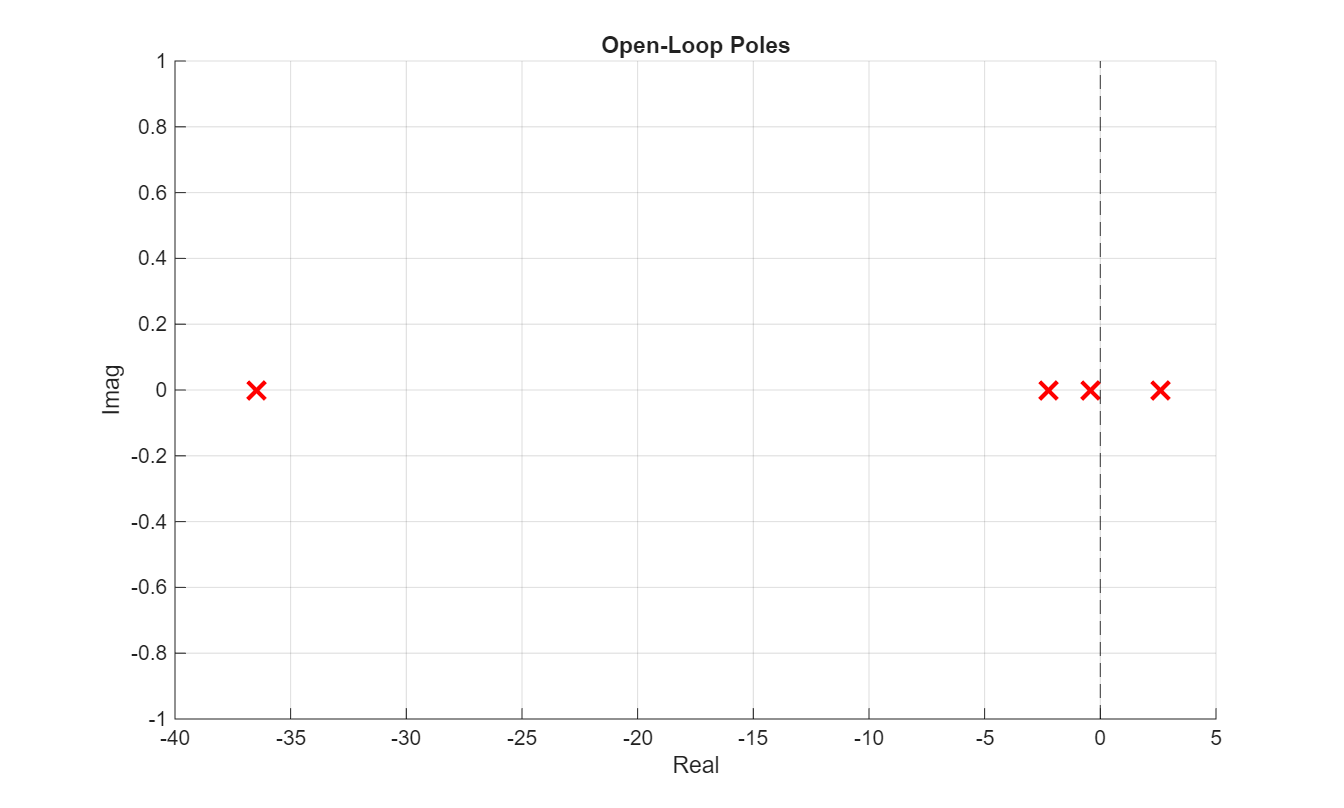
\includegraphics[width=0.6\linewidth]{../figures/OL-Poles.png}
	\caption{Open-loop pole map. The pole in the right half-plane is the seesaw fall rate $p_{OL}$ and is the design driver for the closed-loop bandwidth.}
	\label{fig:ol_poles}
\end{figure}

\paragraph{$p_{1,2}$: Dominant balancing mode.} Poles $p_{1,2}$ govern the unstable angular dynamics.
\begin{itemize}
	\item \textbf{Decay rate $\sigma_{th}$:} Set to $4.5$ rad/s, approximately twice the open-loop divergence rate. This makes the linear closed-loop response faster than the natural fall dynamics without requiring unnecessarily high gain.
	\item \textbf{Damping $\zeta_{th}$:} Set to $0.8$. The equivalent second-order overshoot is about $1.5\%$, but the actual overshoot is verified from the complete state-space simulation.
\end{itemize}

\paragraph{$p_3, p_4$: Non-dominant modes.} These real poles are placed further left than the dominant pair so that they do not introduce slower transients.
\begin{itemize}
	\item $p_3 = -6.75$ rad/s: a faster real pole used to damp the cart-velocity component of the response.
	\item $p_4 = -5.4$ rad/s: a real pole used to return the cart toward the centre while keeping the controller less aggressive than a much faster placement.
\end{itemize}

\paragraph{Final pole set and gain.}
\begin{equation}
	p_{\mathrm{des}} = \{-4.5 \pm j3.37,\; -6.75,\; -5.4\} \quad \Rightarrow \quad \mathbf{K} = \begin{bmatrix} 147.43 & 9.83 & -111.00 & -36.71 \end{bmatrix}
\end{equation}

\subsubsection{Resulting gain and verification}

The gain vector $\mathbf{K}$ is computed by \texttt{place}$(A,B,p_{\mathrm{des}})$. Numerical values and simulation checks are produced by \texttt{pole\_placement\_design.m}:
\begin{equation}
	\mathbf{K} = \begin{bmatrix} 147.43 & 9.83 & -111.00 & -36.71 \end{bmatrix}. \T\B
\end{equation}

\begin{figure}[H]
	\centering
	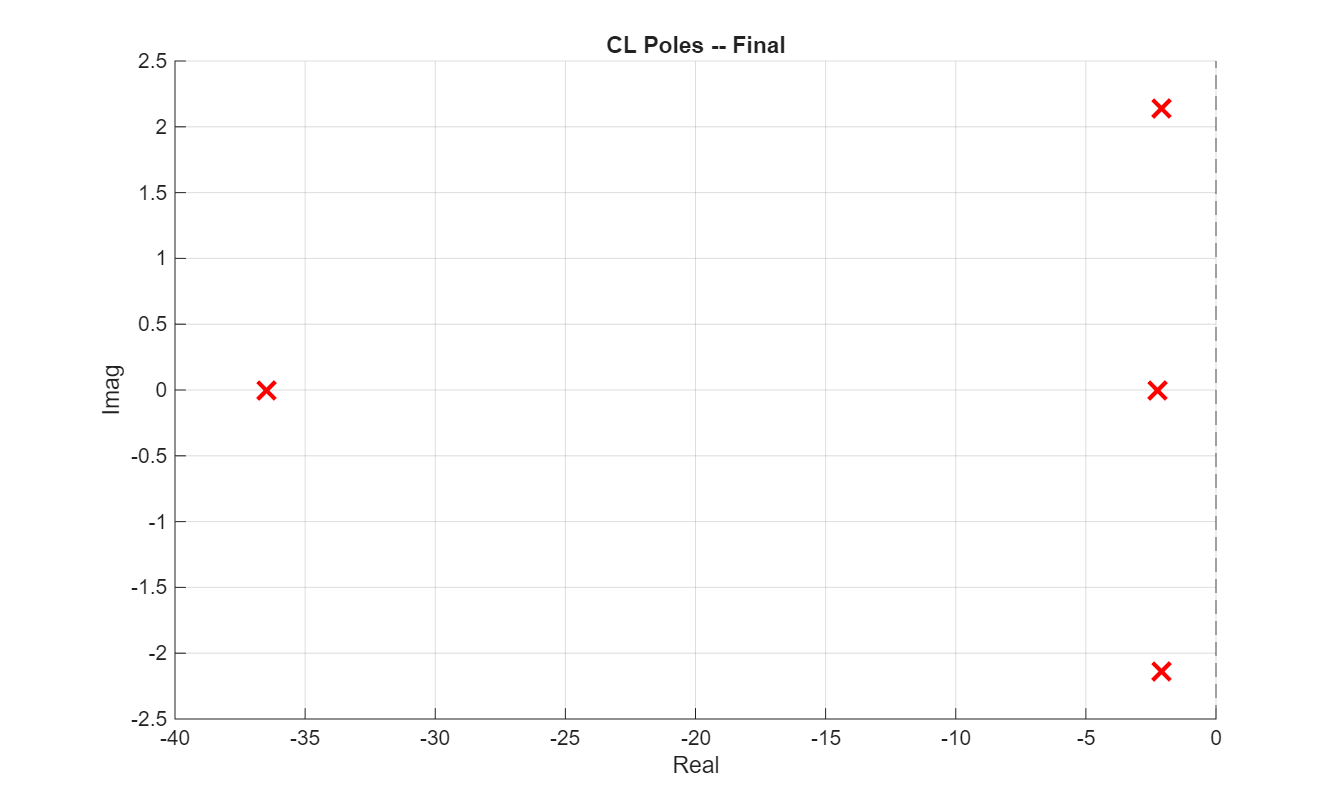
\includegraphics[width=0.6\linewidth]{../figures/CL-Poles-Final.png}
	\caption{Closed-loop poles of the identified linear model. The complex pair is closest to the imaginary axis and is therefore the intended dominant mode. The real poles are faster, so they should not set the slowest linear transient.}
	\label{fig:cl_poles_final}
\end{figure}

The initial-condition test uses $\theta(0) = 2^\circ$ (Fig.~\ref{fig:ic_final}). This is a small-angle test inside the linearisation region and close to a realistic manual startup error. Peak values from the linear simulation are:
\begin{equation*}
	V_m = 3.87\;\text{V}, \qquad \theta = 2.55^\circ, \qquad x_c = 3.26\;\text{cm}.
\end{equation*}
These values are inside the nominal limits of $\pm 6$ V and $\pm 11.5^\circ$. In the linear simulation, the peak voltage scales with the initial angle, giving $\theta_{\max} = 3.10^\circ$ before $V_m$ reaches saturation. Above this value the actuator saturation changes the closed-loop dynamics, so the assigned poles no longer describe the actual response. The $3.10^\circ$ value is therefore a conservative bound for the unsaturated linear regime, not a guarantee of recovery for larger disturbances.

\begin{figure}[H]
	\centering
	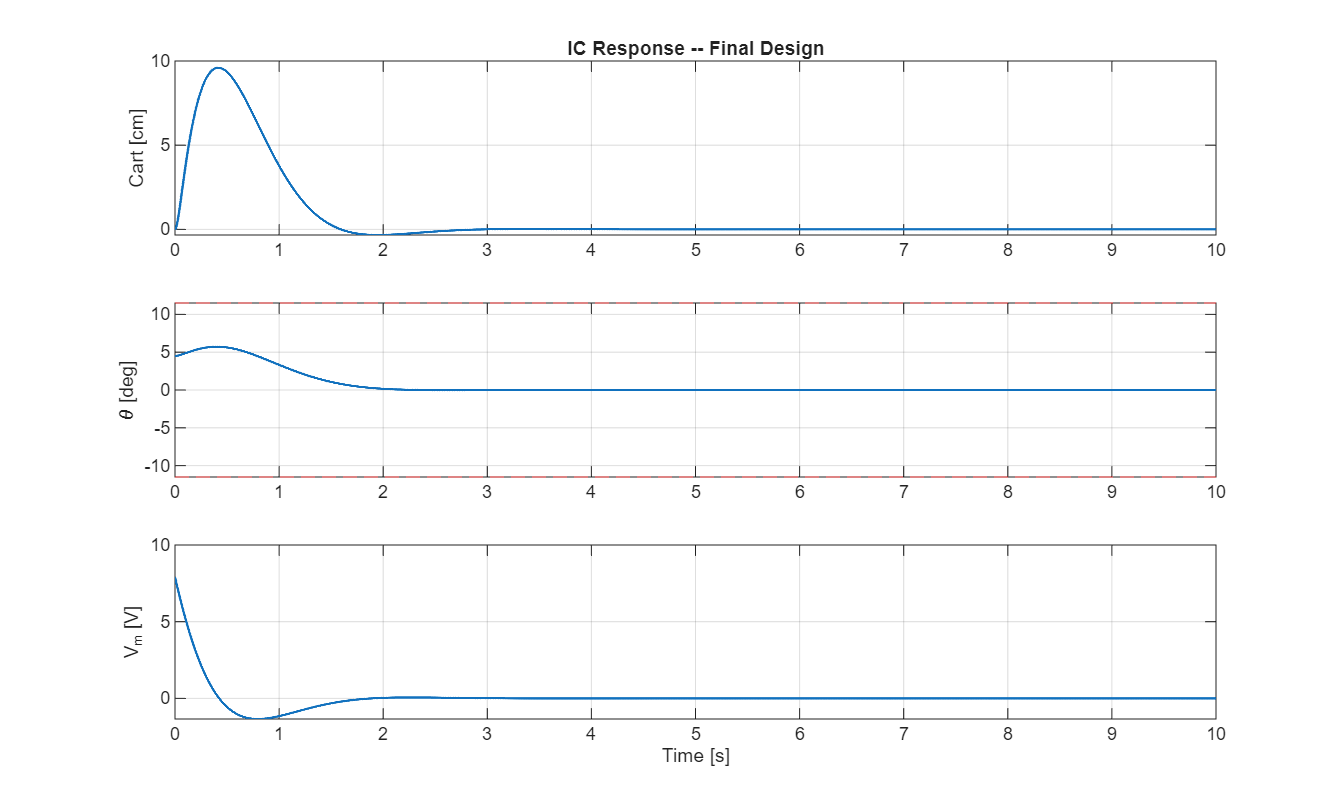
\includegraphics[width=0.8\linewidth]{../figures/IC-Response-Final.png}
	\caption{IC response to $\theta(0) = 2^\circ$. Peak $V_m = 3.87$ V, peak $\theta = 2.55^\circ$, peak cart $= 3.26$ cm.}
	\label{fig:ic_final}
\end{figure}

\subsubsection{Steady-state bias analysis}
\label{sssec:bias}

An off-centre mass of 100 g induces a constant torque $\tau_{bias} \approx 0.123$ Nm. Pure state feedback does not include a disturbance model or integral state, so a constant torque bias produces a nonzero equilibrium angle $\theta_{ss}$ (Fig.~\ref{fig:rep_final}). On hardware, friction and quantisation can turn this offset into a bounded oscillation around a shifted centre.

\begin{figure}[H]
	\centering
	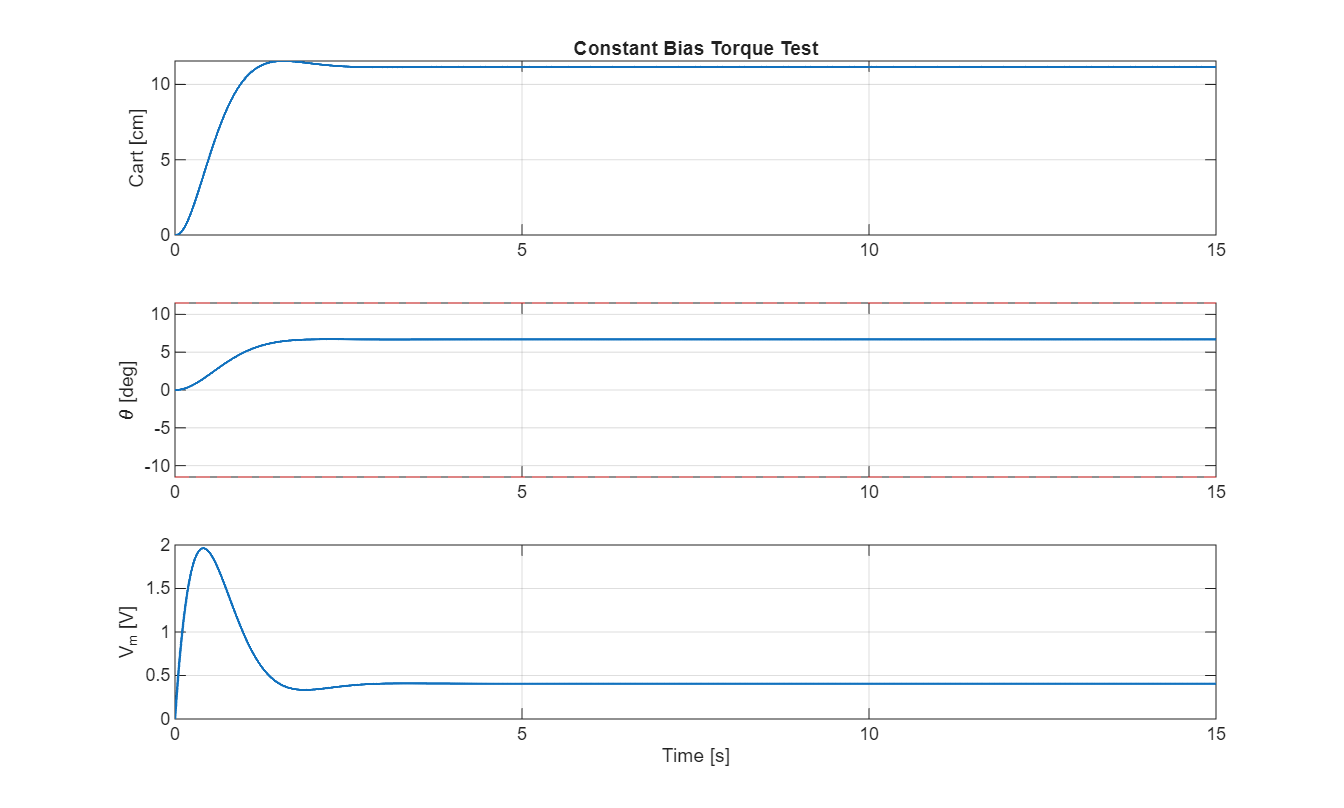
\includegraphics[width=0.8\linewidth]{../figures/repeated_disturbance.png}
	\caption{Response to constant torque bias without integral action. Steady-state error $\theta_{ss}$ shifts the limit-cycle center.}
	\label{fig:rep_final}
\end{figure}

\subsubsection{Integral action}

The state is augmented with $\dot{\xi} = \theta$ to eliminate steady-state error:
\begin{equation}
	\mathbf{x}_a = \begin{bmatrix} x_c & \dot{x}_c & \theta & \dot{\theta} & \xi \end{bmatrix}^\top.
\end{equation}
An integrator pole is placed at $p_{int} = -0.5$ rad/s. The integral state rejects constant torque bias in the linear model by driving the average angle back to zero. It should not be interpreted as removing the hardware limit cycle itself; it mainly shifts the centre of the bounded motion back toward $\theta=0$.

\begin{figure}[H]
	\centering
	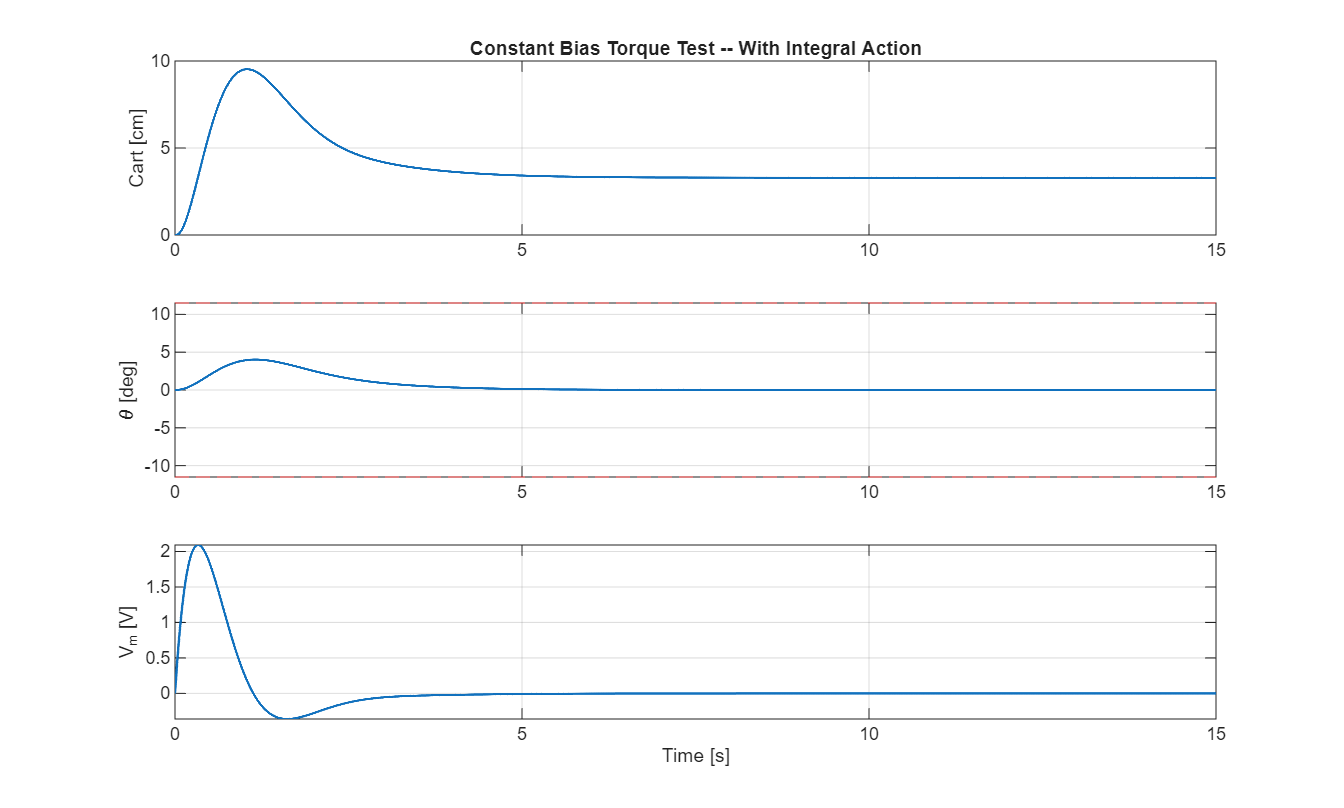
\includegraphics[width=0.8\linewidth]{../figures/bias_with_integral.png}
	\caption{Bias-load response with integral action. Steady-state error is eliminated; oscillation is centered on zero.}
	\label{fig:bias_integral}
\end{figure}

\subsubsection{Frequency-domain validation}

For state feedback there is no unique scalar open-loop transfer function unless the loop-breaking point is specified. The reported frequency plot uses the loop broken at the plant input,
\begin{equation}
	L(s) = \mathbf{K}(sI - A)^{-1}B.
\end{equation}
The Bode and Nyquist plots are therefore local linear robustness checks for this specific loop opening. They are useful for comparing gain and phase margins of the implemented design, but they are not a substitute for hardware validation with saturation, quantisation, and observer dynamics present. On the real setup, the corresponding controller frequency response can be estimated from logged data as $C_{hw}(j\omega) \approx U(j\omega)/E(j\omega)$, where $E$ is the controller input signal and $U$ is the commanded motor voltage.

\begin{figure}[H]
	\centering
	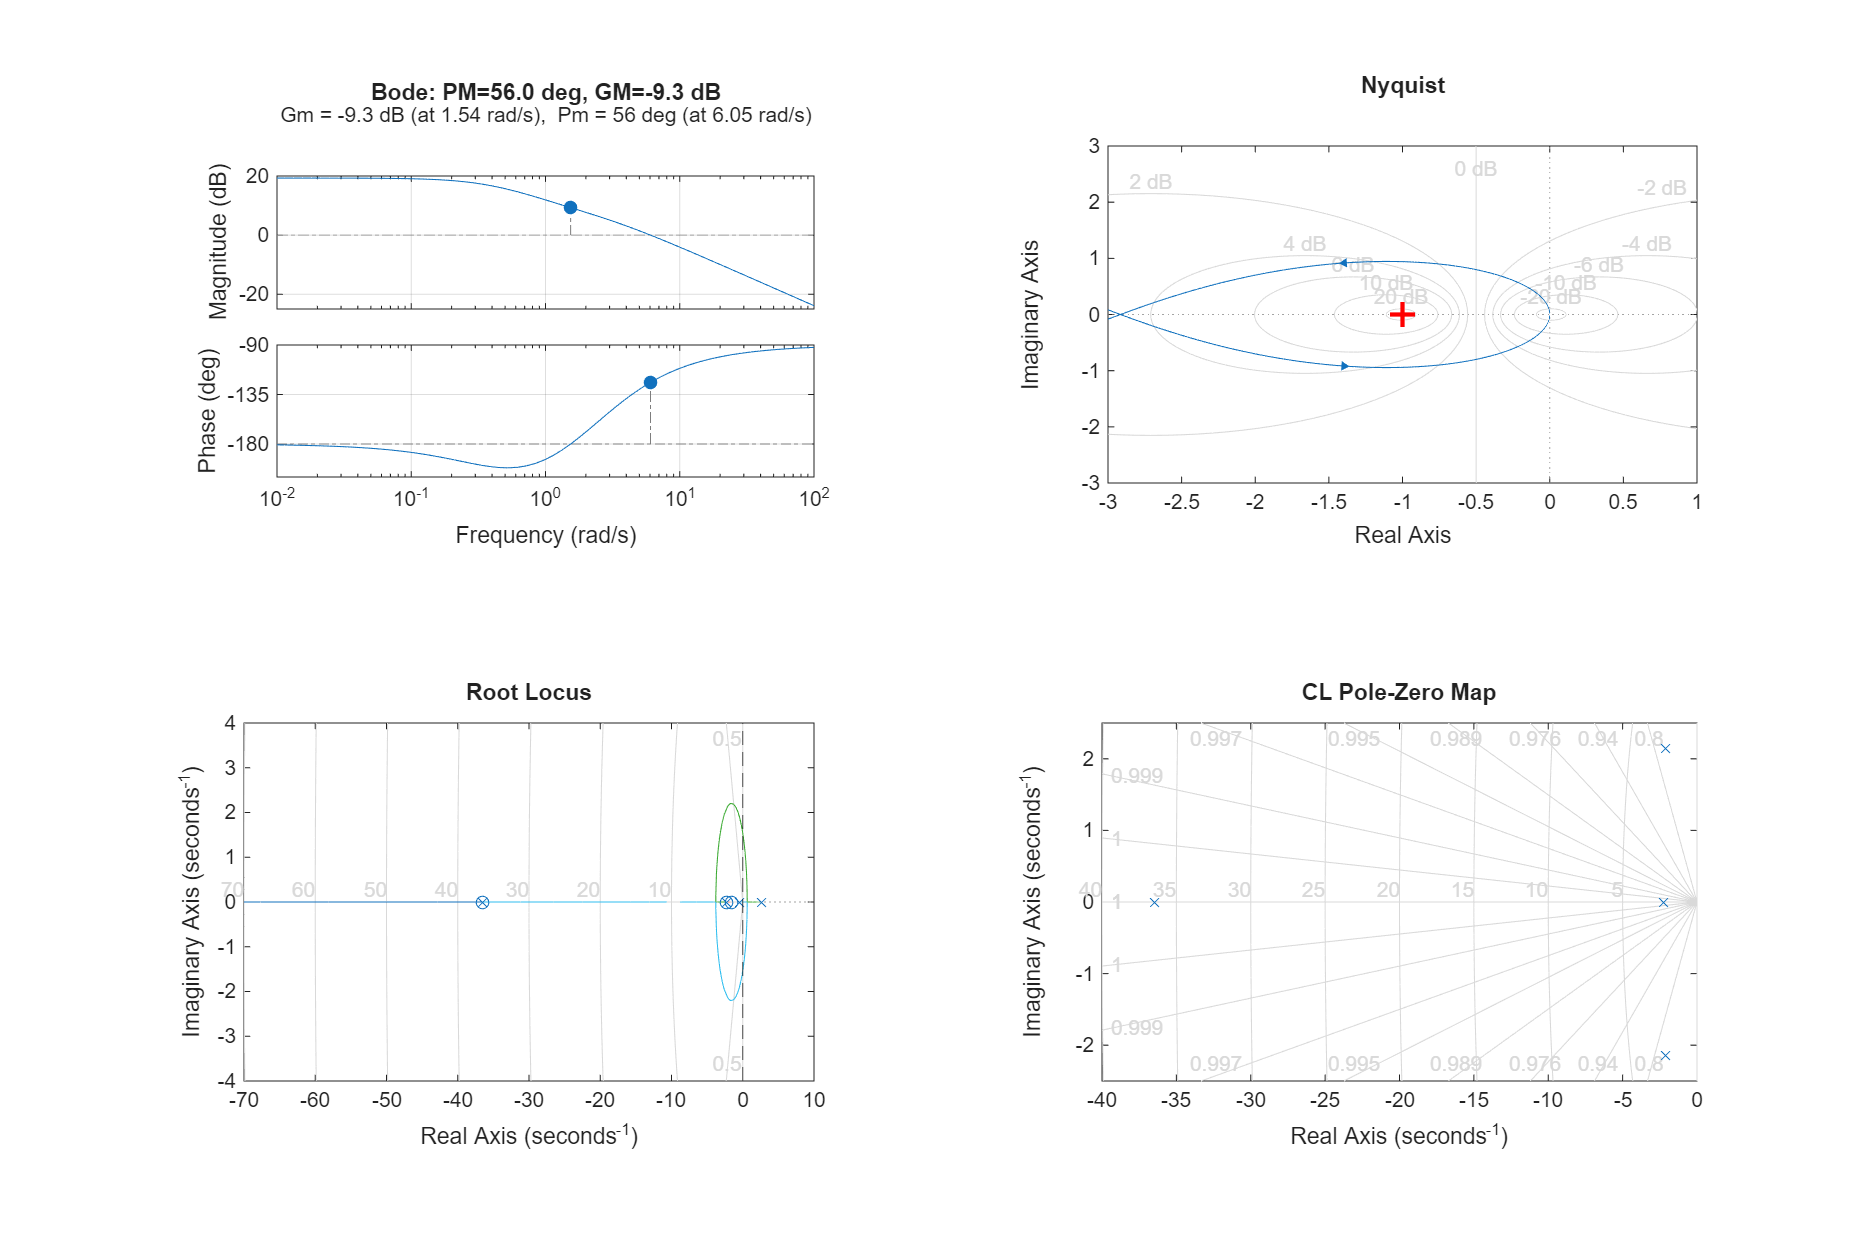
\includegraphics[width=0.9\linewidth]{../figures/loop_analysis.png}
	\caption{Frequency-domain checks for the linear model with the loop broken at the plant input: Bode plot, Nyquist plot, root locus, and closed-loop pole-zero map. These plots support the linear design but do not replace hardware validation.}
	\label{fig:loop_final}
\end{figure}

\subsubsection{Luenberger State Observer}
\label{sssec:observer}

A Luenberger observer is used to estimate the unmeasured states $[\dot{x}_c, \dot{\theta}]$ from position encoders. This replaces numerical differentiation, which introduces significant phase lag.

\paragraph{Theory.}
The measurement matrix is
\begin{equation}
	C_{\mathrm{meas}} = \begin{bmatrix} 1 & 0 & 0 & 0 \\ 0 & 0 & 1 & 0 \end{bmatrix}, \qquad y = C_{\mathrm{meas}}\mathbf{x}.
\end{equation}
The observer
\begin{equation}
	\dot{\hat{\mathbf{x}}} = A\hat{\mathbf{x}} + B u + L\,(y - C_{\mathrm{meas}}\hat{\mathbf{x}})
	\label{eq:luenberger}
\end{equation}
gives an error $e = \mathbf{x} - \hat{\mathbf{x}}$ with dynamics
\begin{equation}
	\dot{e} = (A - L\,C_{\mathrm{meas}})\,e.
	\label{eq:err_dyn}
\end{equation}
$L$ assigns the eigenvalues of $A - LC_{\mathrm{meas}}$ freely whenever $(A, C_{\mathrm{meas}})$ is observable. Closing the loop with $u = -\mathbf{K}\hat{\mathbf{x}}$ gives the block-triangular system
\begin{equation}
	\frac{\mathrm{d}}{\mathrm{d}t}\!\begin{bmatrix} \mathbf{x} \\ e \end{bmatrix}
	= \begin{bmatrix} A - B\mathbf{K} & B\mathbf{K} \\ 0 & A - LC_{\mathrm{meas}} \end{bmatrix}\!\begin{bmatrix} \mathbf{x} \\ e \end{bmatrix},
	\label{eq:separation}
\end{equation}
so $\operatorname{eig}(\cdot) = \operatorname{eig}(A - B\mathbf{K}) \cup \operatorname{eig}(A - LC_{\mathrm{meas}})$ -- the separation principle. Controller and observer decouple, and $\mathbf{K}$ from \S\ref{sec:pole_placement} carries over. The dual identity $\operatorname{eig}(A - LC) = \operatorname{eig}((A^\top - C^\top L^\top)^\top)$ turns the gain problem into pole placement on $(A^\top, C_{\mathrm{meas}}^\top)$, solved with \texttt{place} as for $\mathbf{K}$.

\paragraph{Tuning.}
Let $\sigma_{\mathrm{obs}} = \min_i |\Re(p_{\mathrm{obs},i})|$.

\textit{Lower bound -- separation.} The estimate must settle faster than the controller bandwidth. A standard heuristic
\begin{equation}
	|\Re(p_{\mathrm{obs}})| \;\geq\; (3{-}5)\,|\Re(p_{\mathrm{ctrl}})|
\end{equation}
separates the observer and controller timescales.

\textit{Upper bound -- noise.} An encoder count perturbs the input by $\delta V_m = \mathbf{K} L\,\delta y$. With quanta
\begin{equation}
	q_{x_c} = K_{ec} \approx 2.28\times 10^{-5}\,\text{m},
	\qquad q_\theta = K_{E,SW}/K_{gs} \approx 5.0\times 10^{-4}\,\text{rad},
\end{equation}
the per-count voltage chatter has a budget $|\mathbf{K} L|_i\,q_i \lesssim 0.1$ V on each channel. $L$ inflates with $k_{\mathrm{obs}}$, and so does this product.

\textit{Damping.} Internal to the error dynamics. Mirror the controller pair, $\zeta = 0.8$.

\textit{Sweep.} Evaluating the noise gain across the target range:
\begin{table}[H]
	\centering
	\begin{tabular}{c|cc|c}
		\hline
		\rowcolor{bluePoli!40}
		$k_{\mathrm{obs}}$ & $|\mathbf{K}L|_1\,q_{x_c}$ [V/count] & $|\mathbf{K}L|_2\,q_\theta$ [V/count] & $t_{\mathrm{settle}}$ [s] \T\B \\
		\hline
		\hline
		1.50 & 0.000 & 2.40 & 1.02 \T\\
		\textbf{2.00} & \textbf{0.190} & \textbf{0.055} & \textbf{0.84} \\
		2.50 & 0.171 & 3.71 & 0.64 \\
		3.00 & 0.148 & 6.93 & 0.54 \\
		3.50 & 0.118 & 9.56 & 0.46 \\
		4.00 & 0.547 & 8.25 & 0.43 \B\\
		\hline
	\end{tabular}
	\caption{Observer-gain sweep. The $\theta$-channel noise gain is negligible at $k_{\mathrm{obs}} = 2.0$ ($0.055$ V/count), then jumps to $3.71$ V/count at $k_{\mathrm{obs}} = 2.5$ -- the noise-gain knee. Cold-start at $k_{\mathrm{obs}} = 2.5$ exceeds $V_{sat}$ ($8.54$ V peak), ruling out higher values.}
	\label{table:kobs_sweep}
\end{table}

The range $k_{\mathrm{obs}} \geq 2.5$ is unsuitable: the $\theta$-channel noise gain exceeds the chatter budget and cold-start saturation occurs. We pick $k_{\mathrm{obs}} = 2.0$, just below the noise-gain knee:
\begin{equation}
	p_{\mathrm{obs}} = 2.0 \cdot \{\,-4.5 \pm j3.37,\; -6.75,\; -5.4\,\} = \{\,-9.0 \pm j6.75,\; -13.5,\; -10.8\,\}.
\end{equation}
This gives a $2\times$ separation ratio. The slowest observer pole at $-9.0$ rad/s is $3\times$ the unstable open-loop pole ($+3.03$ rad/s), satisfying the functional separation requirement.

\paragraph{Verification.}
The design script \texttt{luenberger\_observer\_design.m} runs all six checks. Numerical results for the chosen $k_{\mathrm{obs}} = 2.0$:
\begin{enumerate}
	\item \textbf{Observability.} $\operatorname{rank}(\mathcal{O}) = 4$, $\operatorname{cond}(\mathcal{O}) = 3.7\times 10^{2}$ -- well-conditioned. Both states behind each encoder (velocity behind position, $\dot\theta$ behind $\theta$) are recoverable.
	\item \textbf{Gain.}
	\begin{equation}
		L = \begin{bmatrix} 23.72 & -12.88 \\ -71.75 & 69.97 \\ 29.71 & -0.20 \\ 214.08 & -35.42 \end{bmatrix}.
	\end{equation}
	The dominant entries are in the $x_c$ column for the velocity rows and the $\theta$ column for $\dot\theta$ -- the dynamic coupling drives the correction.
	The error dynamics decouple from the controller by construction. Eigenvalue mismatch between the combined $8\times 8$ matrix and the union of controller/observer spectra: $8.7\times 10^{-14}$, i.e.\ machine precision.
	\item \textbf{IC error decay.} A realistic initial condition of $\theta(0) = 2^\circ$ is used for validation. With $\hat{\mathbf{x}}(0)=0$ and $\mathbf{x}(0) = [0,0,2^\circ,0]^\top$, all four error components fall inside their encoder-quantum tolerance by $t = 0.90$ s, consistent with the slowest observer pole at $-9.0$ rad/s.
	\item \textbf{Loop in the loop.} The combined system response is plotted in Fig.~\ref{fig:obs_ic}.
	\item \textbf{Noise injection.}
	\begin{equation}
		|\mathbf{K} L|_1\,q_{x_c} = 0.19\;\text{V/count}, \qquad
		|\mathbf{K} L|_2\,q_\theta = 0.055\;\text{V/count}.
	\end{equation}
	The $\theta$-channel gain matches the controller-only $V_{chatter} = 0.055$ V/count -- the observer introduces essentially zero additional noise amplification in this channel.
\end{enumerate}

\paragraph{Noise and bandwidth trade-off.}
At $k_{\mathrm{obs}} = 2.0$, the $\theta$-channel noise gain is $0.055$ V/count, matching the full-state baseline. The observer bandwidth ($\approx 9$ rad/s) is three orders of magnitude below the sampling rate (1 kHz), so encoder quantisation noise is not passed directly into the control input. On hardware this must be validated against a differentiated encoder signal and a causally low-pass filtered differentiated signal; the expected advantage of the observer is a smoother velocity estimate without the delay required by an aggressively filtered differentiator.

\paragraph{Startup transient.}
The observer is validated for a $2.0^\circ$ startup excursion. Peak transient values are compared in Table~\ref{table:obs_startup}.

\begin{table}[H]
	\centering
	\begin{tabular}{lcc}
		\hline
		\rowcolor{bluePoli!40}
		Configuration & peak $V_m$ [V] & peak $\theta$ [deg] \T\B \\
		\hline\hline
		Full-state controller (baseline) & 3.87 & 2.55 \T\\
		Observer (cold start, $\hat{\mathbf{x}}(0)=0$) & 6.40 & 2.98 \\
		Observer (realistic initialization) & 3.87 & 2.55 \B\\
		\hline
	\end{tabular}
	\caption{Transient peak comparison ($\theta(0)=2^\circ$). Cold-start voltage exceeds $V_{sat}$. Realistic initialization is required for hardware deployment.}
	\label{table:obs_startup}
\end{table}

The natural deployment is to seed the observer with the encoders at the moment the controller starts:
\begin{equation}
	\hat{\mathbf{x}}(0) = \begin{bmatrix} x_{c,\mathrm{meas}} & 0 & \theta_{\mathrm{meas}} & 0 \end{bmatrix}^\top,
	\label{eq:obs_init}
\end{equation}
zeroing only the unmeasured velocities. With this initialisation the only nonzero error component is the initial velocity guess error (zero in this scripted IC, small in practice), and the observer is transparent: the closed-loop voltage and angle traces match the full-state controller-alone case. Cold-starting from $\hat{\mathbf{x}}(0)=0$ slightly exceeds $V_{sat}$ ($6.40$ V peak), so the realistic initialisation from encoder readings is mandatory for safe startup.

\begin{figure}[H]
	\centering
	
\includegraphics[width=0.6\linewidth]{../figures/Observer-Poles.png}
	\caption{Observer poles (blue) vs controller poles (red). The dominant theta-loop pair sits $2\times$ further left than the controller's; all observer poles are well into the LHP, with the slowest at $-9.0$ rad/s.}
	\label{fig:obs_poles}
\end{figure}

\begin{figure}[H]
	\centering
	\includegraphics[width=0.85\linewidth]{../figures/Observer-IC-Response.png}
	\caption{Cold-start IC response with the observer in the loop at $\theta(0) = 2^\circ$. The cart peaks at $3.3$ cm, $\theta$ overshoots to $3.0^\circ$ (well inside the $\pm 11.5^\circ$ stops, dashed red), and $V_m$ peaks at $6.40$ V, slightly exceeding the saturation envelope (dashed red). With the realistic initialisation \eqref{eq:obs_init} the voltage trace drops to the controller-only profile (peak $3.87$ V).}
	\label{fig:obs_ic}
\end{figure}

\paragraph{Note on the augmented controller.}
With integral action the controller state is $\mathbf{x}_a = [\mathbf{x}; \xi]$ where $\dot{\xi} = \theta$. Since $\theta$ is measured directly, $\xi$ is integrated from the encoder reading, not from $\hat{\theta}$. Only the four plant states are estimated; the observer carries over to the augmented controller without modification.

\subsubsection{Implementation and Hardware Results}

On hardware, only $x_c$ and $\theta$ are measured by encoders. The Luenberger observer of \S\ref{sssec:observer} reconstructs $\dot{x}_c$ and $\dot{\theta}$ from the encoder pair using the linearised plant model, replacing the differentiator + low-pass filter scheme.

\paragraph{Verification Protocol.}
The observer is verified sequentially to ensure model fidelity:
\begin{enumerate}
    \item \textbf{Open-Loop Tracking:} Verify $\hat{\dot{x}}_c, \hat{\dot{\theta}}$ convergence during manual displacement with $V_m = 0$.
    \item \textbf{Convergence:} Verify software IC convergence ($\hat{\theta}(0) = 15^\circ$) against simulation.
    \item \textbf{Noise Assessment:} Monitor steady-state motor vibration. Excessive oscillation indicates high observer bandwidth requiring gain reduction.
\end{enumerate}

% TODO: Simulink block diagram screenshot
% TODO: Hardware test — initial tilt response (plot + table: settling time, peak theta, peak V_m)
% TODO: Hardware test — bias load response with integral action
% TODO: Compare simulation vs hardware results, discuss discrepancies

\subsection{AI-Assisted Rapid Prototyping of Robust Controllers}
\label{sec:ai_robust_prototyping}

The pole-placement controller and the integral-action extension are both derived from the local linear model. In practice, however, the measured seesaw response showed the same qualitative limitation for several linear designs: instead of converging asymptotically to $\theta=0$, the hardware settles into a bounded rocking motion. The preceding bias-load study already shows that integral action can recenter the average angle, but it does not remove the hardware limit cycle itself. Since the identified model had proven unreliable outside small local predictions, the next step was not to commit immediately to one controller family, but to rapidly prototype several robust alternatives and compare them on a common nonlinear benchmark.

This exploration was carried out with AI-assisted scripting. The useful role of the AI tool was not to replace control-design judgement, but to accelerate the repetitive parts of the study: generating candidate synthesis scripts, wiring each controller into the same simulation harness, collecting comparable metrics, and quickly discarding controllers that failed the nonlinear constraints. The final decision remains based on the physical metrics: peak-to-peak rocking, voltage effort, voltage slew rate, saturation, and survival under motor-protection limits.

\subsubsection{Nonlinear limit-cycle simulation}
\label{sssec:nonlinear_limit_cycle_sim}

The robust-controller benchmark uses the identified linear matrices $A_{sw},B_{sw}$ as the nominal plant, but inserts the main non-ideal hardware effects in the simulation loop. The state-feedback controller receives quantised encoder measurements
\begin{equation}
    x_{c,q} = q_x \operatorname{round}\!\left(\frac{x_c}{q_x}\right), \qquad
    \theta_q = q_\theta \operatorname{round}\!\left(\frac{\theta}{q_\theta}\right),
\end{equation}
where $q_x = K_{ec}$ and $q_\theta = K_{E,SW}/K_{gs}$. The motor command is then passed through saturation, deadzone, and asymmetric drive gain:
\begin{equation}
    u_s = \operatorname{sat}(u,\pm 6\,\mathrm{V}), \qquad
    u_d =
    \begin{cases}
        0, & |u_s| < 0.12\,\mathrm{V},\\
        u_s - 0.12\operatorname{sign}(u_s), & |u_s| \geq 0.12\,\mathrm{V},
    \end{cases}
\end{equation}
\begin{equation}
    u_{eff} =
    \begin{cases}
        1.0\,u_d, & u_d \geq 0,\\
        0.5\,u_d, & u_d < 0.
    \end{cases}
\end{equation}
A Coulomb-friction disturbance is added in the cart acceleration channel,
\begin{equation}
    d_f = \begin{bmatrix}0 & -F_c\operatorname{sign}(\dot{x}_c)/M_c & 0 & 0\end{bmatrix}^\top,
    \qquad F_c = 0.18\,\mathrm{N},
\end{equation}
and the simulated cart and seesaw are clamped at the physical rail and angle limits. This combination introduces the same mechanism observed on hardware: close to zero angle, the requested voltage often lies inside the deadzone, quantisation prevents infinitesimal feedback corrections, Coulomb friction produces stick--slip motion, and the asymmetric actuator gain biases the two half-cycles. The result is a bounded limit cycle rather than exact convergence.

The baseline pole-placement controller reproduces the large rocking effect in this benchmark. With the same $2^\circ$ initial release used in the controller tests, the simulated pole-placement steady-state rocking is $3.38^\circ$ peak-to-peak, matching the order of the hardware observation and motivating the robust-controller comparison.

\subsubsection{Controllers compared}

The benchmark in \texttt{scripts/analysis/robust\_controller\_comparison.m} evaluates the following controller families on the same nonlinear plant:
\begin{itemize}
    \item pole-placement state feedback, used as the baseline;
    \item an LMI-certified state-feedback gain, where high-performing candidates are checked by common quadratic Lyapunov inequalities over uncertainty vertices;
    \item an $H_\infty$ Riccati state-feedback design;
    \item an actuator-aware $H_\infty$ design with an augmented actuator-voltage state to penalise aggressive voltage motion;
    \item super-twisting sliding-mode control (SMC) with a boundary layer;
    \item a softened scheduled SMC variant;
    \item a Takagi--Sugeno fuzzy gain scheduler implemented using the Fuzzy Logic Toolbox.
\end{itemize}
True dynamic \texttt{hinfsyn} controllers were also attempted after installing the Robust Control Toolbox. Although the resulting dynamic controllers were linearly stabilising, none survived the nonlinear deadzone and constraint validation from the $2^\circ$ release without falling into saturation or an angle stop. They were therefore excluded from the final surviving-controller table rather than reported as valid.

\begin{figure}[H]
    \centering
    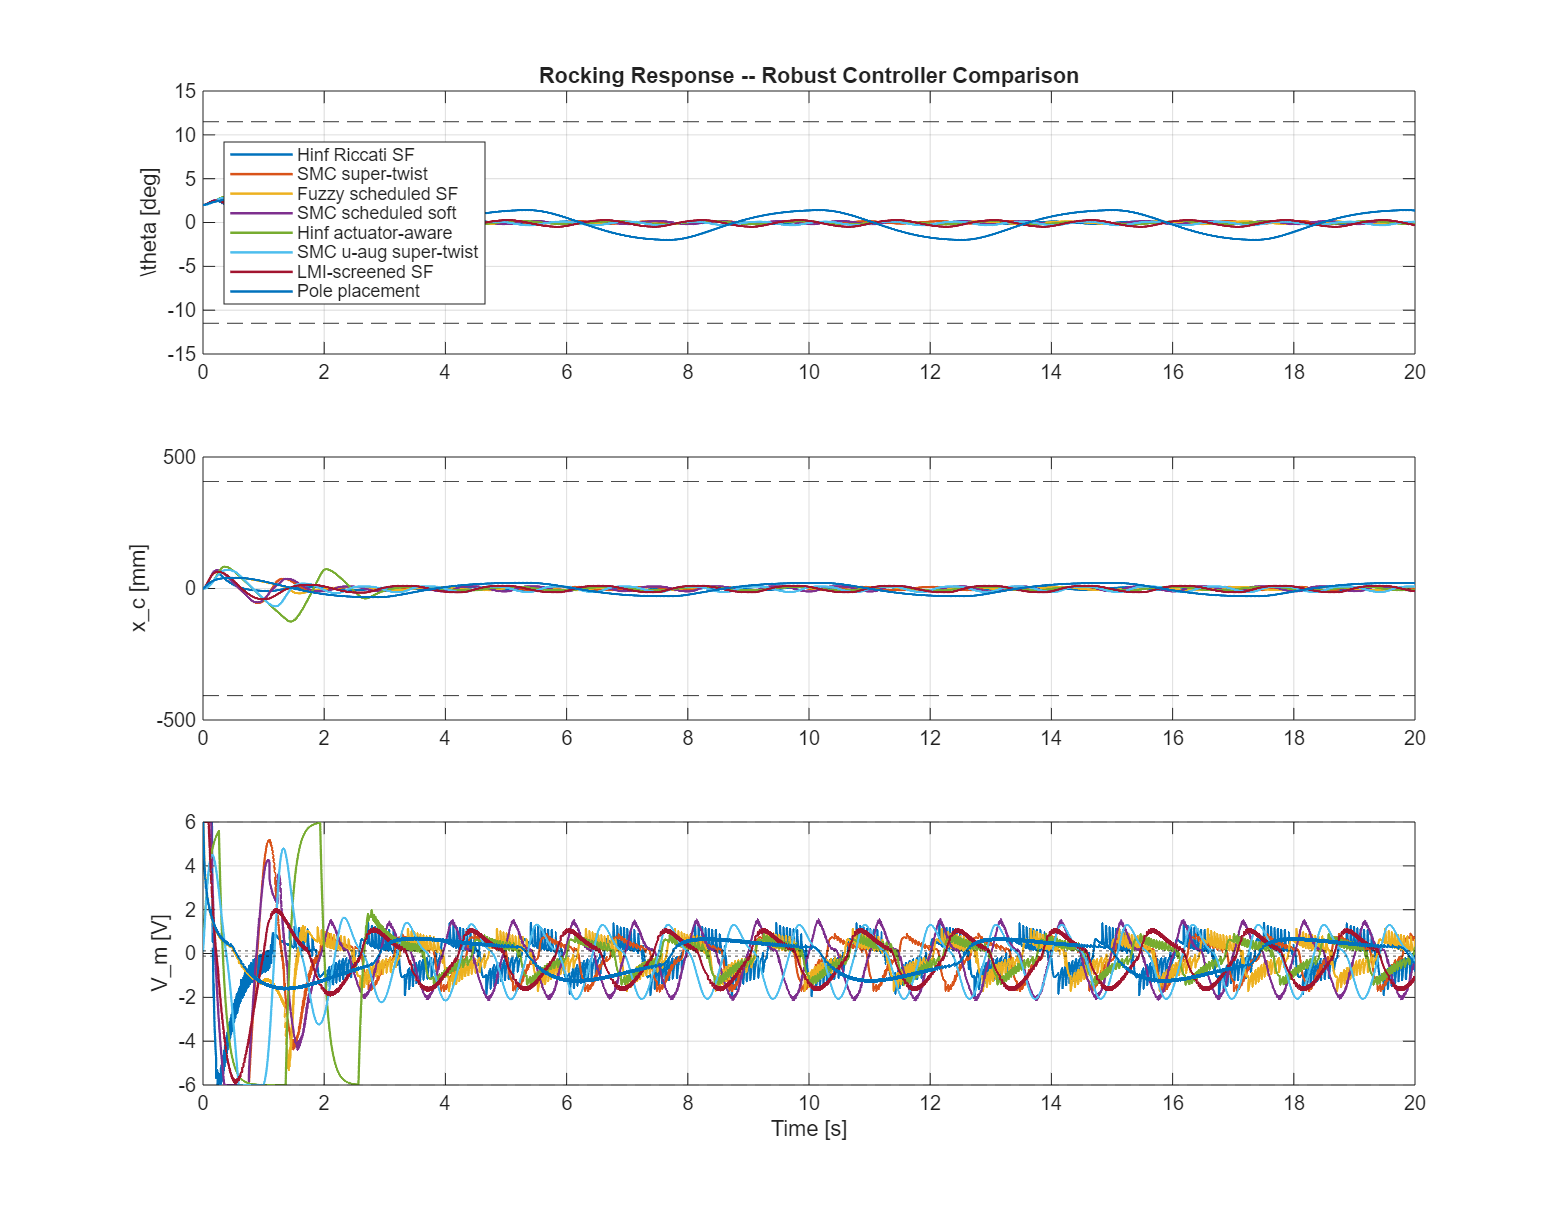
\includegraphics[width=0.95\linewidth]{../figures/Robust-Control-Comparison.png}
    \caption{AI-assisted robust-controller comparison on the nonlinear limit-cycle benchmark. All controllers are simulated with the same quantisation, deadzone, asymmetric actuator gain, Coulomb friction, saturation, and stops.}
    \label{fig:robust_comparison}
\end{figure}

\begin{figure}[H]
    \centering
    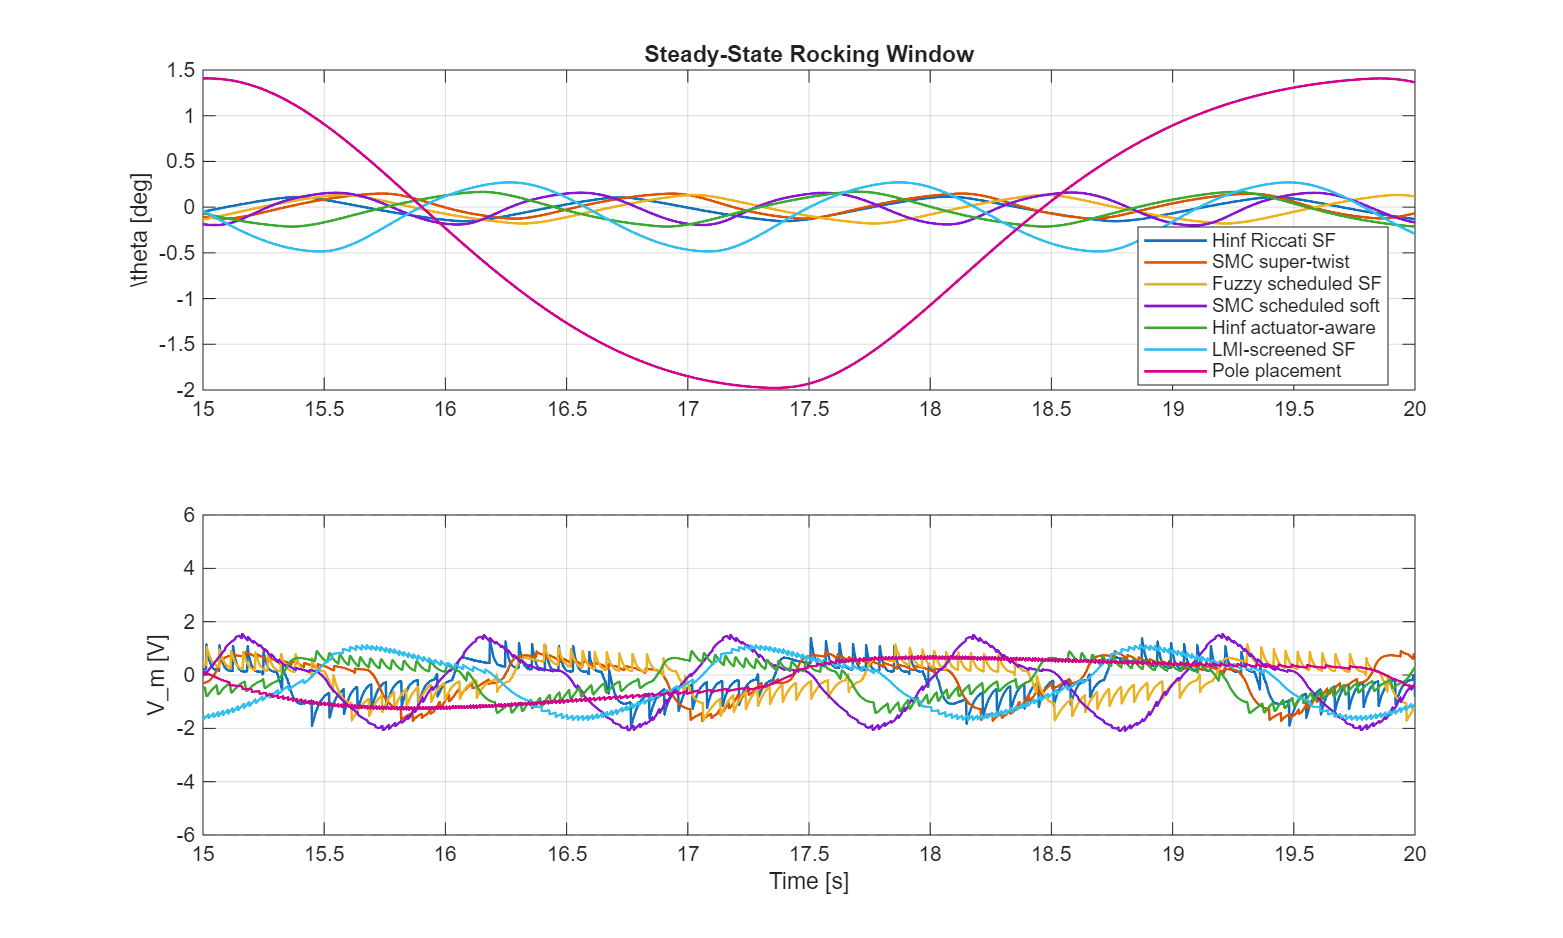
\includegraphics[width=0.95\linewidth]{../figures/Robust-Control-SteadyState.png}
    \caption{Steady-state rocking window for the robust-controller comparison. The pole-placement controller keeps the plant bounded but leaves a much larger oscillation envelope than the robust candidates.}
    \label{fig:robust_steady_state}
\end{figure}

\begin{figure}[H]
    \centering
    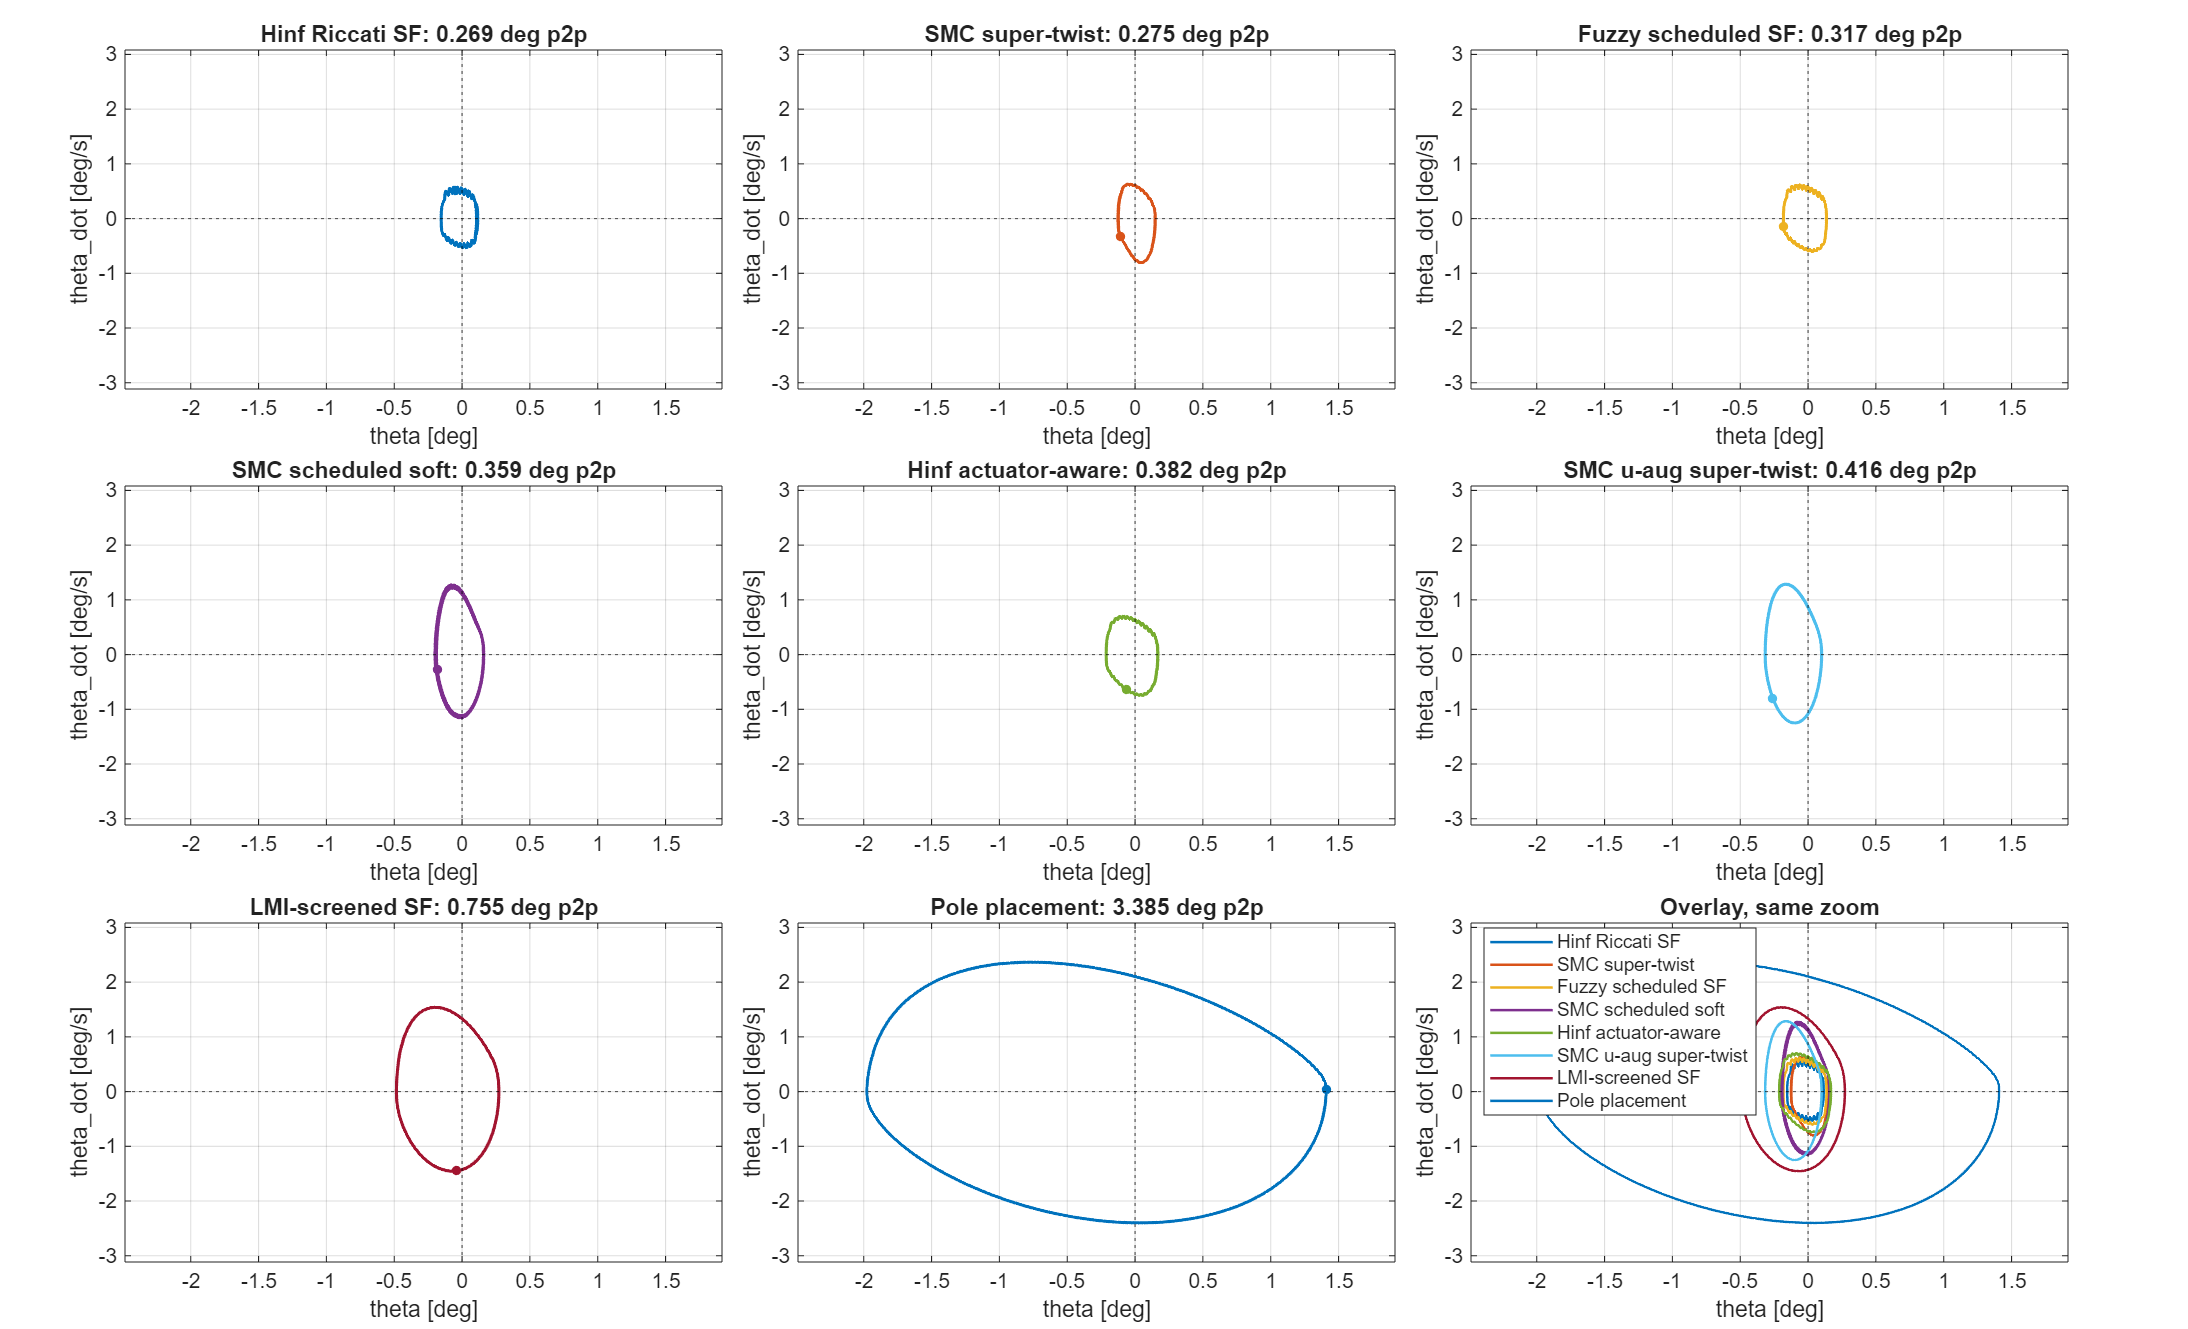
\includegraphics[width=0.95\linewidth]{../figures/Robust-Control-ThetaPhasePlane.png}
    \caption{Steady-state phase-plane portraits, $\theta$ versus $\dot\theta$, for the robust-controller candidates. The plot visualises the remaining limit cycles after the transient has decayed.}
    \label{fig:robust_phase_plane}
\end{figure}

\subsubsection{Nominal nonlinear benchmark results}

Table~\ref{table:robust_nominal_metrics} reports the final comparison metrics over the last five seconds of a 20 s simulation. The primary objective is minimising $\theta$ peak-to-peak; control effort and voltage slew are treated as secondary hardware-stress metrics.

\begin{table}[H]
    \centering
    \resizebox{\textwidth}{!}{%
    \begin{tabular}{lcccccc}
        \hline
        \rowcolor{bluePoli!40}
        Controller & OK & $\theta_{pp}$ [deg] & $\theta_{rms}$ [deg] & $u_{rms}$ [V] & $u_{pk}$ [V] & peak slew [V/s] \T\B \\
        \hline\hline
        $H_\infty$ Riccati SF & yes & 0.269 & 0.087 & 0.662 & 6.000 & 654.8 \T\\
        SMC super-twist & yes & 0.275 & 0.095 & 0.759 & 6.000 & 270.2 \\
        Fuzzy scheduled SF & yes & 0.312 & 0.104 & 0.638 & 6.000 & 338.5 \\
        SMC scheduled soft & yes & 0.359 & 0.124 & 1.127 & 6.000 & 609.3 \\
        $H_\infty$ actuator-aware & yes & 0.382 & 0.132 & 0.640 & 6.000 & 120.0 \\
        LMI-screened SF & yes & 0.755 & 0.280 & 0.967 & 6.000 & 108.9 \\
        Pole placement & yes & 3.385 & 1.235 & 0.726 & 6.000 & 153.6 \B\\
        \hline
    \end{tabular}}
    \caption{Nominal nonlinear robust-controller benchmark. Metrics are computed on the steady-state window $t\geq15$ s.}
    \label{table:robust_nominal_metrics}
\end{table}

The best nominal peak-to-peak result is obtained by the $H_\infty$ Riccati state-feedback controller, closely followed by the super-twisting SMC. However, both achieve this by allowing relatively aggressive voltage changes. The actuator-aware $H_\infty$ controller is more hardware-friendly: it increases the angle envelope to $0.382^\circ$ peak-to-peak but reduces the peak voltage slew to approximately $120$ V/s and avoids saturation in the nominal run. The LMI-screened controller also has a low slew requirement, but at the cost of a larger $0.755^\circ$ oscillation.

\subsubsection{Motor-protection and slew-rate survival}

To evaluate weak-hardware operation, the same controllers were tested with an explicit voltage slew-rate limiter. This is not intended as the final design method; it is a stress test showing which controllers remain viable if the motor amplifier must be protected from fast voltage changes. Table~\ref{table:robust_slew_survival} gives the lowest slew-rate limit at which each controller still satisfies the simulation constraints.

\begin{table}[H]
    \centering
    \begin{tabular}{lccc}
        \hline
        \rowcolor{bluePoli!40}
        Controller & lowest surviving limit [V/s] & $\theta_{pp}$ [deg] & $u_{rms}$ [V] \T\B \\
        \hline\hline
        Pole placement & 10 & 3.421 & 0.767 \T\\
        Fuzzy scheduled SF & 35 & 0.341 & 0.643 \\
        LMI-screened SF & 50 & 0.760 & 0.978 \\
        $H_\infty$ Riccati SF & 100 & 0.280 & 0.616 \\
        $H_\infty$ actuator-aware & 100 & 0.382 & 0.661 \\
        SMC super-twist & 100 & 0.273 & 0.766 \\
        SMC scheduled soft & 100 & 0.360 & 1.116 \B\\
        \hline
    \end{tabular}
    \caption{Slew-rate survival test. The reported row is the lowest voltage slew limit for which the controller remains within the nonlinear simulation constraints.}
    \label{table:robust_slew_survival}
\end{table}

\begin{figure}[H]
    \centering
    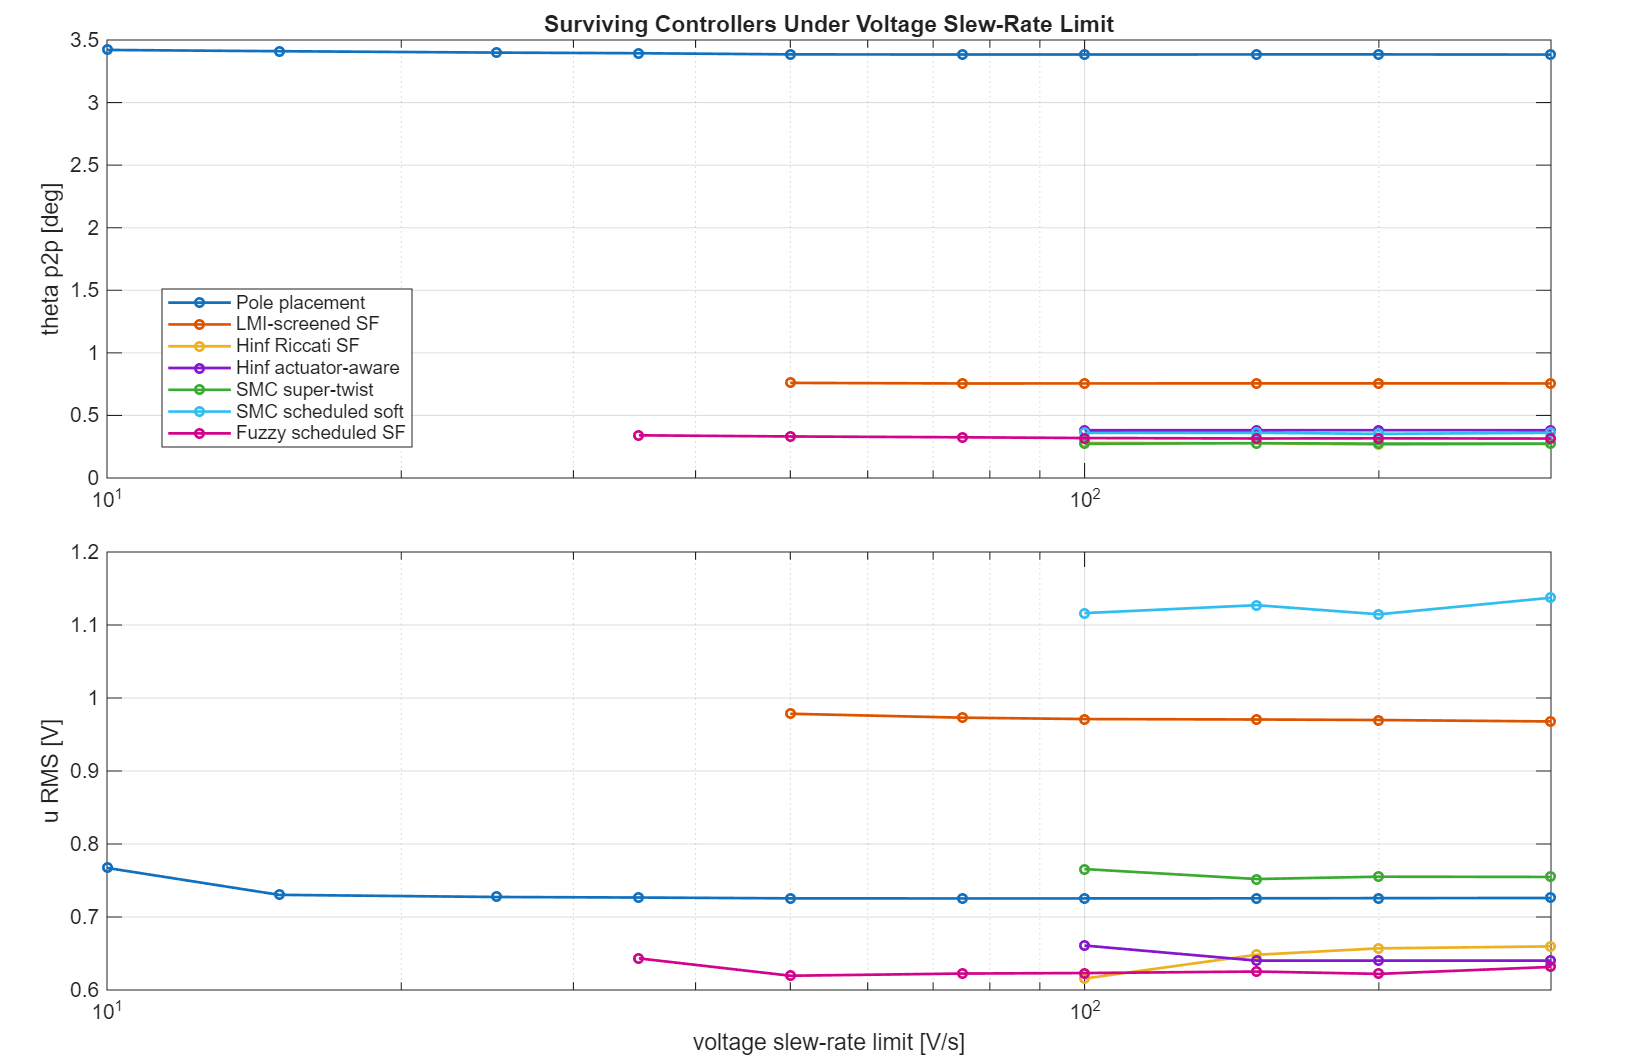
\includegraphics[width=0.95\linewidth]{../figures/Robust-Control-RateLimitSurvival.png}
    \caption{Controller survival under voltage slew-rate limits. Fuzzy scheduling is the best low-slew robust candidate: it remains below $0.35^\circ$ peak-to-peak at 35 V/s, while the more aggressive $H_\infty$ and SMC candidates require about 100 V/s.}
    \label{fig:robust_rate_limit}
\end{figure}

The low-slew test changes the preferred controller. If the hardware can tolerate slew rates of approximately $100$ V/s or higher, the $H_\infty$ Riccati and SMC controllers give the smallest angle envelopes. If the design priority is weak-hardware protection, the fuzzy scheduled controller is more attractive: it is the best surviving robust controller at 75, 50, and 35 V/s, with $\theta_{pp}=0.341^\circ$ at 35 V/s. Below that level only the pole-placement controller survives in this benchmark, but it returns to the original large limit cycle of approximately $3.4^\circ$ peak-to-peak.

Based on these results, the most promising next hand-designed controller is the fuzzy scheduled state-feedback law. It does not give the absolute smallest nominal peak-to-peak angle, but it offers the best compromise between strong rocking suppression and low voltage slew-rate requirements. The next design step is therefore to replace the automatically swept fuzzy scheduler by an explicitly engineered rule base, using the robust-comparison results as the target envelope.

\section{Experience 3: Lift-off supervisor and catch from rest}
\label{sec:liftoff}

\subsection{Motivation}

The pole-placement controller of Section~\ref{sec:pole_placement} is designed for the locally linearised plant about the upright equilibrium $\theta=0$. In normal hardware operation the seesaw rests against one of the mechanical stops at $\theta = \pm \alpha_{\max} \approx \pm 11.5^\circ$, which lies just outside the validity envelope of the linear model. Engaging the pole-placement gain $\mathbf{K}_{pp}$ directly from the resting stop is unreliable: the cart-position contribution $-K_{pp,1}\,x_c$ alone demands tens of volts because the encoder-zero is not the cart's resting position, the requested voltage immediately saturates, the pinion gear slips against the rack, and the closed-loop guarantees of the linear design no longer apply.

To bridge from the resting stop to the linear-regime equilibrium, a two-mode supervisor is introduced: a \emph{lift-off} mode that gently brings the state inside the basin of attraction of the linear controller, and a \emph{balance} mode that takes over once that basin is reached. The handoff between the two is governed by a Lyapunov sublevel set of the closed-loop pole-placement design.

\subsection{Supervisor architecture}
\label{ssec:liftoff_supervisor}

The supervisor switches between two state-feedback laws applied to the same plant:
\begin{equation}
    u(t) = \begin{cases}
        -\mathbf{K}_{lift}\,\mathbf{x}(t), & \text{if } c(t) = 0,\\
        -\mathbf{K}_{pp}\,\mathbf{x}(t),  & \text{if } c(t) = 1,
    \end{cases}
    \qquad
    \mathbf{K}_{lift} = \beta\,\mathbf{K}_{pp}, \quad \beta \in (0,1).
\end{equation}
The Boolean $c(t)$ is a one-way catch latch driven by a Lyapunov gating test described below. The reduced gain $\beta\,\mathbf{K}_{pp}$ provides the same direction of control action as the balance controller but at a fraction of the magnitude, so the initial voltage demand at $\theta=\theta_{\max}$ stays below $V_{sat}$ and avoids the saturation slam that produces pinion slip on the hardware.

\paragraph{Lyapunov catch criterion.}
Let $A_{cl} = A_{sw} - B_{sw}\mathbf{K}_{pp}$ denote the closed-loop dynamics matrix of the balance controller. Because $\mathbf{K}_{pp}$ is stabilising on the linear model, $A_{cl}$ is Hurwitz, and for any $Q \succ 0$ the Lyapunov equation
\begin{equation}
    A_{cl}^{\top} P + P A_{cl} = -Q
    \label{eq:lyap_eq}
\end{equation}
admits a unique positive-definite solution $P \succ 0$. The quadratic form
\begin{equation}
    V(\mathbf{x}) = \mathbf{x}^{\top} P \,\mathbf{x}
    \label{eq:lyap_V}
\end{equation}
is then a Lyapunov function for the balance closed-loop near the origin: along trajectories of $\dot{\mathbf{x}}=A_{cl}\mathbf{x}$, $\dot V = -\mathbf{x}^{\top}Q\mathbf{x} \leq 0$, with equality only at $\mathbf{x}=\mathbf{0}$. Sublevel sets $\{\mathbf{x}:V(\mathbf{x})\le c\}$ are therefore positively invariant on the linear model, and small enough sublevel sets are also invariant on the saturated nonlinear closed loop.

The catch latch fires once $V(\mathbf{x})$ drops below a design threshold $c_{catch}$ and remains set thereafter:
\begin{equation}
    c(t) = c(t^-) \;\lor\; \big[\,V(\mathbf{x}(t)) < c_{catch}\,\big], \qquad c(0)=0.
    \label{eq:catch_latch}
\end{equation}
The one-way latch prevents chattering between modes if $V(\mathbf{x})$ briefly recrosses the threshold during the post-handoff transient. The threshold is sized relative to the Lyapunov value at the resting state $\mathbf{x}_{rest} = [0,0,\alpha_{\max},0]^\top$:
\begin{equation}
    V_{rest} = \mathbf{x}_{rest}^{\top} P \,\mathbf{x}_{rest},
    \qquad
    c_{catch} = V_{rest}/3.
    \label{eq:c_catch}
\end{equation}
Choosing $c_{catch}$ as a fraction of $V_{rest}$ guarantees that the lift-off must drive the state at least three times closer to the origin (in the Lyapunov metric) before the linear controller is allowed to take over.

\paragraph{Design constants.}
With $Q = \operatorname{diag}(1,\,0.1,\,10,\,1)$ and the identified plant from \S\ref{sec:pole_placement}, the supervisor constants are
\begin{align}
    \mathbf{K}_{pp}   &= \begin{bmatrix} +226.5 & +18.9 & -197.9 & -63.2 \end{bmatrix}, \\
    \beta             &= 0.30, \qquad
    \mathbf{K}_{lift} = \begin{bmatrix} +67.9 & +5.68 & -59.4 & -18.9 \end{bmatrix}, \\
    V_{rest}          &= 0.726,\qquad
    c_{catch}         = 0.242.
\end{align}

\subsection{Manual calibration procedure}
\label{ssec:liftoff_calibration}

In the test reported below the encoder zero of $\theta$ was set with the seesaw held manually at the upright equilibrium and the motor command at zero. The sequence was:
\begin{enumerate}
    \item start the QUARC model with $V_m = 0$;
    \item hold the seesaw at $\theta \approx 0$ by hand for a few seconds while the encoder logs an offset-free zero reference;
    \item with $V_m$ still at zero, release the seesaw so it settles against one of the mechanical stops at $\theta = -\alpha_{\max}$;
    \item engage the supervisor: the lift-off mode begins driving the cart, the Lyapunov test gates the handoff to the balance controller, and the closed-loop response is logged through the standard \texttt{To Host File} block.
\end{enumerate}
This procedure removes the cart's encoder-zero ambiguity but does not remove the cart's physical offset from the rail centre at the moment the seesaw drops onto its stop. The data shows the consequence: at controller engage the cart has slid downhill under gravity to the low end of the rail.

\subsection{Hardware results}
\label{ssec:liftoff_results}

Figure~\ref{fig:liftoff_timeline} shows the entire $295.9$ s session. The supervisor was started at $t = 27.32$ s with the seesaw on the negative stop, and the run includes several caught windows (green-shaded). Their durations are not a performance metric -- they reflect when the operator chose to manually return the seesaw to the stop and restart, not when the controller would have failed on its own. Only the \emph{first} catch is reported in detail below, because the catch latch (\ref{eq:catch_latch}) is one-way: once it trips, the lift-off gain $\mathbf{K}_{lift}$ is no longer active. Subsequent catches in the same session correspond to the balance controller re-entering its basin from a new initial condition, not to the lift-off design itself.

\begin{figure}[H]
    \centering
    \includegraphics[width=0.95\linewidth]{../figures/HW-Liftoff-File2-Timeline.png}
    \caption{Hardware lift-off run, $295.9$ s. The red vertical line marks the first controller engage at $t = 27.32$ s; this is the only event in the session at which the lift-off gain $\mathbf{K}_{lift}$ acted. Subsequent green-shaded windows are the balance controller re-entering its basin after a manual re-release of the seesaw and do not exercise the lift-off design. The voltage trace shows the characteristic ``hammering'' limit cycle of the pole-placement controller in steady state.}
    \label{fig:liftoff_timeline}
\end{figure}

Figure~\ref{fig:liftoff_catch_zoom} zooms on the first lift-off and catch event. The controller engages at $t = 27.32$ s with the seesaw on the negative stop ($\theta = -11.66^\circ$) and the cart at the high end of the rail ($x_c = +0.43$ m, slid downhill from the encoder-zero position). The lift-off mode commands a saturated negative voltage; the cart accelerates downhill of the rail's reference frame, crosses the pivot near $x_c \approx 0$, and the seesaw rotates through upright. At $t \approx 28.2$ s the Lyapunov score $V(\mathbf{x})$ falls below $c_{catch} = 0.242$, the latch trips, and the balance controller engages with a brief overshoot, then settles into the standard rocking limit cycle. The bottom panel shows $V(\mathbf{x})$ on a logarithmic scale: it decreases by more than two decades during the lift-off and stabilises around $V \sim 10^{-2}$ in the balance regime.

\begin{figure}[H]
    \centering
    \includegraphics[width=0.92\linewidth]{../figures/HW-Liftoff-File2-Catch.png}
    \caption{Catch zoom on the first lift-off episode. The red dashed line is the controller-engage instant. The green dashed line marks the moment when $V(\mathbf{x})$ crosses below the catch threshold $c_{catch} = V_{rest}/3$ and the supervisor switches from $\mathbf{K}_{lift}$ to $\mathbf{K}_{pp}$. The cart sweeps from $+43$ cm to a slight overshoot at $-13$ cm during the lift-off, then settles near zero.}
    \label{fig:liftoff_catch_zoom}
\end{figure}

The steady-state behaviour following the first catch is characterised in Figure~\ref{fig:liftoff_steady} over the window $t = 31.5\text{--}59.5$ s -- the first catch window with $3$ s trimmed at the start (catch transient) and $0.5$ s trimmed at the end (operator-initiated release back to the stop). The angle histogram shows the bimodal signature of the limit cycle, with peaks near $0^\circ$ and $-1.5^\circ$ and a mean offset of $-0.71^\circ$ caused by the deadzone--Coulomb asymmetry of the actuator (no integral action is used in this supervisor variant). The cart position oscillates within roughly $\pm 2$ cm of its mean and the voltage command stays comfortably inside $\pm 6$ V throughout the window, with no sustained saturation.

\begin{figure}[H]
    \centering
    \includegraphics[width=0.95\linewidth]{../figures/HW-Liftoff-File2-SteadyState.png}
    \caption{Steady-state limit cycle following the first catch ($t = 31.5\text{--}59.5$ s; the catch transient and the operator's terminal release are trimmed). Left column: time traces of $\theta$, $x_c$, and $V_m$; right column: the corresponding distributions. The bimodal $\theta$ histogram is the expected signature of the deadzone--Coulomb limit cycle.}
    \label{fig:liftoff_steady}
\end{figure}

Figure~\ref{fig:liftoff_phase} aggregates the full run in two views. The phase plane $(\theta, \dot\theta)$ is colour-coded by time: the early lift-off episodes (cool colours) trace large loops that reach the stops, while the later balance episodes (warm colours) concentrate near the origin. The Lyapunov trace on the right separates the same data into bands: $V(\mathbf{x}) > V_{rest}$ when the seesaw is on a stop, an intermediate region during each lift-off, and $V(\mathbf{x}) \in [10^{-4}, 10^{-1.5}]$ in the caught regime, comfortably below $c_{catch}$.

\begin{figure}[H]
    \centering
    \includegraphics[width=0.95\linewidth]{../figures/HW-Liftoff-File2-PhaseLyap.png}
    \caption{Left: phase plane $(\theta, \dot\theta)$ for the full run, coloured by time. Early lift-off attempts (cool colours) explore the full angle range; the caught regime (warm colours) concentrates near the origin. Right: Lyapunov score $V(\mathbf{x}) = \mathbf{x}^{\top}P\mathbf{x}$ over the run; the red and green dashed lines are $V_{rest}$ and $c_{catch}$ respectively.}
    \label{fig:liftoff_phase}
\end{figure}

Table~\ref{table:liftoff_metrics} summarises the limit-cycle metrics over the trimmed post-catch window. Peak and peak-to-peak values are reported as the $5\text{--}95$ percentile range so a single end-of-window outlier (the operator-initiated release back to the stop) does not dominate the figure.

\begin{table}[H]
    \centering
    \begin{tabular}{lc}
        \hline
        \rowcolor{bluePoli!40}
        Metric & Value \T\B \\
        \hline\hline
        $\theta$ peak-to-peak ($5\text{--}95$ pct)   & $1.52^\circ$ \T\\
        $\theta$ peak-to-peak ($1\text{--}99$ pct)   & $1.58^\circ$ \\
        $|\theta|$ ($95$ pct)                          & $1.43^\circ$ \\
        $\theta$ mean (bias)                           & $-0.71^\circ$ \\
        $\theta$ RMS (about mean)                      & $0.60^\circ$ \\
        $x_c$ mean                                     & $-1.20$ cm \\
        $x_c$ peak-to-peak ($5\text{--}95$ pct)        & $3.74$ cm \\
        $V_m$ RMS                                      & $2.09$ V \\
        $|V_m|$ ($95$ pct)                             & $4.39$ V \B\\
        \hline
    \end{tabular}
    \caption{Limit-cycle metrics in the trimmed steady-state window after the first catch ($t = 31.5\text{--}59.5$ s, $28$ s). Percentile-based statistics are used to keep one-sample end-of-window outliers from dominating the peak-to-peak figures.}
    \label{table:liftoff_metrics}
\end{table}

\subsection{Discussion}

The hardware run validates two properties of the supervisor design and exposes a limitation.

First, the Lyapunov-gated handoff (\ref{eq:catch_latch}) is a workable catch criterion on the physical system. During the first lift-off the score $V(\mathbf{x})$ decreased monotonically from $V_{rest} \approx 0.73$ to below $c_{catch} = 0.24$ over roughly $0.9$ s, the latch tripped, and the balance controller engaged with only the small overshoot visible in Figure~\ref{fig:liftoff_catch_zoom}.

Second, the reduced-gain lift-off mode bridged from the resting stop without producing pinion slip on the rack. With $\beta = 0.30$ the cart-position term still saturates briefly at the start of the lift-off, but the saturation episode is short and the resulting peak current did not unseat the gear on the cart drive in this run.

The principal limitation is that only the first catch in the session is informative for the lift-off design. The latch is one-way, so once it trips, $\mathbf{K}_{lift}$ is no longer in the loop. The subsequent caught windows in Figure~\ref{fig:liftoff_timeline} are therefore not lift-off events: they are the balance controller recovering from intermediate initial conditions after a manual re-release. A fair characterisation of $\mathbf{K}_{lift}$ requires either a sequence of independent runs each starting from the rest stop, or a supervisor extension that resets the latch when $V(\mathbf{x})$ exceeds a hysteretic upper threshold so a new lift-off can begin automatically. The second option is also a prerequisite for robustness to large external disturbances and is left as a topic for future work.

The residual steady-state bias of $-0.71^\circ$ in the angle (Table~\ref{table:liftoff_metrics}) is not a supervisor defect: it is the same deadzone--Coulomb asymmetry that drives the limit cycle of the pole-placement controller itself, and would be removed by the integral-action variant of $\mathbf{K}_{pp}$ described in \S\ref{sec:pole_placement} at the cost of a slightly more elaborate handoff condition involving the integral state.

\begin{comment}
	%-----------------------------------------------------------------------------
	% INTRODUCTION
	%-----------------------------------------------------------------------------
	\section{Introduction}
	\label{sec:introduction}
	This document is intended to be both an example of the Polimi \LaTeX{} template for Master Theses in article format,
	as well as a short introduction to its use. It is not intended to be a general introduction to \LaTeX{} itself,
	and the reader is assumed to be familiar with the basics of creating and compiling \LaTeX{} documents (see \cite{oetiker1995not, kottwitz2015latex}).
	\\
	The cover page of the thesis in article format must contain all the relevant information:
	title of the thesis, name of the Study Programme, name(s) of the author(s),
	student ID number, name of the supervisor, name(s) of the co-supervisor(s) (if any), academic year.
	\\
	Be sure to select a title that is meaningful.
	It should contain important keywords to be identified by indexer.
	Keep the title as concise as possible and comprehensible even to people who are not experts in your field.
	The title has to be chosen at the end of your work so that it accurately captures the main subject of the manuscript.

	It is convenient to break the article format of your thesis (in article format) into sections and subsections.
	If necessary, subsubsections, paragraphs and subparagraphs can be used.
	A new section is created by the command
	\begin{verbatim}
\section{Title of the section}
\end{verbatim}
	The numbering can be turned off by using \verb|\section*{}|.
	A new subsection is created by the command
	\begin{verbatim}
\subsection{Title of the subsection}
\end{verbatim}
	and, similarly, the numbering can be turned off by adding an asterisk as follows
	\begin{verbatim}
\subsection*{}
\end{verbatim}
	It is recommended to give a label to each section by using the command
	\begin{verbatim}
\label{sec:section_name}%
\end{verbatim}
	where the argument is just a text string that you'll use to reference that part
	as follows: \textit{Section~\ref{sec:introduction} contains \sc{INTRODUCTION}  \dots}.

	%-----------------------------------------------------------------------------
	% EQUATIONS
	%-----------------------------------------------------------------------------
	\section{Equations}
	\label{sec:eqs}
	This section gives some examples of writing mathematical equations in your thesis.

	Maxwell's equations read:
	\begin{subequations}
		\label{eq:maxwell}
		\begin{align}[left=\empheqlbrace]
			\nabla\cdot \bm{D}                                         & = \rho, \label{eq:maxwell1}   \\
			\nabla \times \bm{E} +  \frac{\partial \bm{B}}{\partial t} & = \bm{0}, \label{eq:maxwell2} \\
			\nabla\cdot \bm{B}                                         & = 0, \label{eq:maxwell3}      \\
			\nabla \times \bm{H} - \frac{\partial \bm{D}}{\partial t}  & = \bm{J}. \label{eq:maxwell4}
		\end{align}
	\end{subequations}

	Equation~\eqref{eq:maxwell} is automatically labeled by \texttt{cleveref},
	as well as Equation~\eqref{eq:maxwell1} and Equation~\eqref{eq:maxwell3}.
	Thanks to the \verb|cleveref| package, there is no need to use \verb|\eqref|.
	Equations have to be numbered only if they are referenced in the text.

	Equations~\eqref{eq:maxwell_multilabels1}, \eqref{eq:maxwell_multilabels2}, \eqref{eq:maxwell_multilabels3}, and \eqref{eq:maxwell_multilabels4} show again Maxwell's equations without brace:
	\begin{align}
		\nabla\cdot \bm{D}                                         & = \rho, \label{eq:maxwell_multilabels1}   \\
		\nabla \times \bm{E} +  \frac{\partial \bm{B}}{\partial t} & = \bm{0}, \label{eq:maxwell_multilabels2} \\
		\nabla\cdot \bm{B}                                         & = 0, \label{eq:maxwell_multilabels3}      \\
		\nabla \times \bm{H} - \frac{\partial \bm{D}}{\partial t}  & = \bm{J} \label{eq:maxwell_multilabels4}.
	\end{align}

	Equation~\eqref{eq:maxwell_singlelabel} is the same as before,
	but with just one label:
	\begin{equation}
		\label{eq:maxwell_singlelabel}
		\left\{
		\begin{aligned}
			\nabla\cdot \bm{D}                                         & = \rho,   \\
			\nabla \times \bm{E} +  \frac{\partial \bm{B}}{\partial t} & = \bm{0}, \\
			\nabla\cdot \bm{B}                                         & = 0,      \\
			\nabla \times \bm{H} - \frac{\partial \bm{D}}{\partial t}  & = \bm{J}.
		\end{aligned}
		\right.
	\end{equation}

	%-----------------------------------------------------------------------------
	% FIGURES, TABLES AND ALGORITHMS
	%-----------------------------------------------------------------------------
	\section{Figures, Tables and Algorithms}

	Figures, Tables and Algorithms have to contain a Caption that describes their content, and have to be properly referred in the text.

	\subsection{Figures}
	\label{subsec:figures}

	For including pictures in your text you can use \texttt{TikZ} for high-quality hand-made figures \cite{tikz},
	or just include them with the command
	\begin{verbatim}
\includegraphics[options]{filename.xxx}
\end{verbatim}
	Here xxx is the correct format, e.g.  \verb|.png|, \verb|.jpg|, \verb|.eps|, \dots.

	\begin{figure}[H]
		\centering
		
\includegraphics[width=0.3\textwidth]{logo_polimi_scritta.eps}
		\caption{Caption of the Figure.}
		\label{fig:quadtree}
	\end{figure}

	Thanks to the \texttt{\textbackslash subfloat} command, a single figure, such as Figure~\ref{fig:quadtree},
	can contain multiple sub-figures with their own caption and label, e.g. Figure~\ref{fig:polimi_logo1} and Figure~\ref{fig:polimi_logo2}.

	\begin{figure}[H]
		\centering
		\subfloat[One PoliMi logo.\label{fig:polimi_logo1}]{
			
\includegraphics[scale=0.5]{Images/logo_polimi_scritta.eps}
		}
		\quad
		\subfloat[Another one PoliMi logo.\label{fig:polimi_logo2}]{
			
\includegraphics[scale=0.5]{Images/logo_polimi_scritta2.eps}
		}
		\caption[]{Caption of the Figure.}
		\label{fig:quadtree2}
	\end{figure}

	\subsection{Tables}
	\label{subsec:tables}

	Within the environments \texttt{table} and  \texttt{tabular} you can create very fancy tables as the one shown in Table~\ref{table:example}.

	\begin{table}[H]
		\caption*{\textbf{Example of Table (optional)}}
		\centering
		\begin{tabular}{|p{3em} c c c |}
			\hline
			\rowcolor{bluePoli!40}
			              & \textbf{column1} & \textbf{column2} & \textbf{column3} \T\B \\
			\hline \hline
			\textbf{row1} & 1                & 2                & 3 \T\B                \\
			\textbf{row2} & $\alpha$         & $\beta$          & $\gamma$ \T\B         \\
			\textbf{row3} & alpha            & beta             & gamma \B              \\
			\hline
		\end{tabular}
		\\[10pt]
		\caption{Caption of the Table.}
		\label{table:example}
	\end{table}

	You can also consider to highlight selected columns or rows in order to make tables more readable.
	Moreover, with the use of \texttt{table*} and the option \texttt{bp} it is possible to align them at the bottom of the page. One example is presented in Table~\ref{table:exampleC}.

	\begin{table*}[bp]
		\centering
		\begin{tabular}{|p{3em} | c | c | c | c | c | c|}
			\hline
			%    \rowcolor{bluePoli!40}
			              & \textbf{column1} & \textbf{column2} & \textbf{column3} & \textbf{column4} & \textbf{column5} & \textbf{column6} \T\B \\
			\hline \hline
			\textbf{row1} & 1                & 2                & 3                & 4                & 5                & 6 \T\B                \\
			\textbf{row2} & a                & b                & c                & d                & e                & f \T\B                \\
			\textbf{row3} & $\alpha$         & $\beta$          & $\gamma$         & $\delta$         & $\phi$           & $\omega$ \T\B         \\
			\textbf{row4} & alpha            & beta             & gamma            & delta            & phi              & omega \B              \\
			\hline
		\end{tabular}
		\\[10pt]
		\caption{Highlighting the columns}
		\label{table:exampleC}
	\end{table*}

	\subsection{Algorithms}
	\label{subsec:algorithms}

	Pseudo-algorithms can be written in \LaTeX{} with the \texttt{algorithm} and \texttt{algorithmic} packages.
	An example is shown in Algorithm~\ref{alg:var}.
	\begin{algorithm}[H]
		\label{alg:example}
		\caption{Name of the Algorithm}
		\label{alg:var}
		\label{protocol1}
		\begin{algorithmic}[1]
			\STATE Initial instructions
			\FOR{$for-condition$}
			\STATE{Some instructions}
			\IF{$if-condition$}
			\STATE{Some other instructions}
			\ENDIF
			\ENDFOR
			\WHILE{$while-condition$}
			\STATE{Some further instructions}
			\ENDWHILE
			\STATE Final instructions
		\end{algorithmic}
	\end{algorithm}

	\section{Some further useful suggestions}

	Theorems have to be formatted as follows:
	\begin{theorem}
		\label{a_theorem}
		Write here your theorem.
	\end{theorem}
	\textit{Proof.} If useful you can report here the proof.
	\vspace{0.3cm} % Insert vertical space

	Propositions have to be formatted as follows:
	\begin{proposition}
		Write here your proposition.
	\end{proposition}
	\vspace{0.3cm} % Insert vertical space

	How to insert itemized lists:
	\begin{itemize}
		\item first item;
		\item second item.
	\end{itemize}
	How to write numbered lists:
	\begin{enumerate}
		\item first item;
		\item second item.
	\end{enumerate}

	\section{Use of copyrighted material}

	Each student is responsible for obtaining copyright permissions, if necessary, to include published material in the thesis.
	This applies typically to third-party material published by someone else.

	\section{Plagiarism}

	You have to be sure to respect the rules on Copyright and avoid an involuntary plagiarism.
	It is allowed to take other persons' ideas only if the author and his original work are clearly mentioned.
	As stated in the Code of Ethics and Conduct, Politecnico di Milano \textit{promotes the integrity of research,
		condemns manipulation and the infringement of intellectual property}, and gives opportunity to all those
	who carry out research activities to have an adequate training on ethical conduct and integrity while doing research.
	To be sure to respect the copyright rules, read the guides on Copyright legislation and citation styles available
	at:
	\begin{verbatim}
https://www.biblio.polimi.it/en/tools/courses-and-tutorials
\end{verbatim}
	You can also attend the courses which are periodically organized on "Bibliographic citations and bibliography management".

	%-----------------------------------------------------------------------------
	% CONCLUSION
	%-----------------------------------------------------------------------------
	\section{Conclusions}
	\color{black}
	A final section containing the main conclusions of your research/study
	and possible future developments of your work have to be inserted in the section ``Conclusions''.

	\section{Bibliography and citations}
	Your thesis must contain a suitable Bibliography which lists all the sources consulted on developing the work.
	The list of references is placed at the end of the manuscript after the chapter containing the conclusions.
	It is suggested to use the BibTeX package and save the bibliographic references in the file \verb|bibliography.bib|.
	This is indeed a database containing all the information about the references. To cite in your manuscript, use the \verb|\cite{}| command as follows:
	\\
	\textit{Here is how you cite bibliography entries: \cite{knuth74}, or multiple ones at once: \cite{knuth92,lamport94}}.
	\\
	The bibliography and list of references are generated automatically by running BibTeX \cite{bibtex}.

\end{comment}
%-----------------------------------------------------------------------------
% BIBLIOGRAPHY
%-----------------------------------------------------------------------------
\bibliography{bibliography.bib}

\appendix
\section{Appendix A}
If you need to include an appendix to support the research in your thesis, you can place it at the end of the manuscript.
An appendix contains supplementary material (figures, tables, data, codes, mathematical proofs, surveys, \dots)
which supplement the main results contained in the previous sections.

\section{Appendix B}
It may be necessary to include another appendix to better organize the presentation of supplementary material.

\begin{comment}
	%%%%%%%%%%%%%%%%%%%%%%%%%%%%%%%%%%%%%%%%%%%%%%%%%%%%%%%%%%%%%%
	%%     ABSTRACT IN ITALIAN LANGUAGE AND ACKNOWLEDGMENTS     %%
	%%%%%%%%%%%%%%%%%%%%%%%%%%%%%%%%%%%%%%%%%%%%%%%%%%%%%%%%%%%%%%
	\cleardoublepage

	%-----------------------------------------------------------------------------
	% SOMMARIO
	%-----------------------------------------------------------------------------
	\section*{Abstract in lingua italiana}
	Qui va l'Abstract in lingua italiana della tesi seguito dalla lista di parole chiave.
	\vspace{15pt}
	\begin{tcolorbox}[arc=0pt, boxrule=0pt, colback=bluePoli!60, width=\textwidth, colupper=white]
		\textbf{Parole chiave:} qui, le parole chiave, della tesi, in italiano
	\end{tcolorbox}

	%-----------------------------------------------------------------------------
	% ACKNOWLEDGEMENTS
	%-----------------------------------------------------------------------------
	\section*{Acknowledgements}
	Here you might want to acknowledge someone.

\end{comment}

%-------------------------------------------------------------------------
%	END OF YOUR DOCUMENT
%-------------------------------------------------------------------------
\end{document}
